\documentclass[10pt,a4paper]{article}
\usepackage[T1]{fontenc}
\usepackage[utf8]{inputenc}
\usepackage[margin=2cm]{geometry}
\usepackage{helvet}\renewcommand{\familydefault}{\sfdefault}
\usepackage{booktabs,longtable,array,xcolor,colortbl,enumitem,titlesec,graphicx,caption}
\usepackage[hidelinks]{hyperref}
\definecolor{navy}{HTML}{1F3A68}\definecolor{band}{HTML}{EEF2F7}
\titleformat{\section}{\large\bfseries\color{navy}}{}{0pt}{}
\titleformat{\subsection}{\normalsize\bfseries\color{navy}}{}{0pt}{}
\setlist{nosep,leftmargin=1.2em}
\setlength{\parindent}{0pt}\setlength{\parskip}{4pt}
\graphicspath{{results/}}
\begin{document}
\begin{titlepage}\vspace*{3cm}
{\Huge\bfseries\color{navy} Medicine Stock and Prescription Assessment 2026\par}\vspace{8pt}
{\Large\color{navy} Inferential and predictive analysis: findings and interpretation\par}\vspace{14pt}
{\small\color{gray} QMIA 2026 (MoH, RMS, RSSB, CHAI) \textperiodcentered{} CHAI Rwanda analytics team \textperiodcentered{} 5 November 2026 \textperiodcentered{} Draft for technical review\par}
\end{titlepage}
\tableofcontents\newpage

\section{Executive summary}
This report adds inferential statistics and predictive models to the descriptive QMIA 2026 dashboard. It uses the cleaned dataset of 5 November 2026: 266 facilities, 9,628 managed facility $\times$ medicine pairs, 6,006 prescriptions with 14,059 items, and 175 community health workers (CHWs). All confidence intervals account for the clustering of observations within facilities and the stratification by level of care.

\begin{itemize}\item \textbf{The headline estimates are precise.} Managed-product availability is 93.7\% (92.9-94.4) and expected-medicine availability 87.8\% (87.0-88.6). Weighted to the national facility mix, expected availability falls to 77.7\% (75.8-79.6), because health posts, which are about 69\% of facilities nationally, hold fewer of the medicines they are authorised for. Excluding health posts it is 88.7\%.
\item \textbf{A failed delivery is the strongest modifiable predictor of a stock-out.} When a requested order received nothing, 36.9\% of pairs were stocked out the next month, against 2.9\% after a full delivery: adjusted odds ratio 7.62 (4.57-12.70). Not ordering at all also raised the odds (2.64 (1.94-3.61)).
\item \textbf{Stock-outs persist.} A pair out this month had about 117 times the odds of being out next month. A simple rule (''out in July'') identifies 66.7\% of August stock-outs; a machine-learning model adds value mainly by ranking new risk (AUC 0.73 among pairs not out in July).
\item \textbf{Record accuracy is a facility problem, not a medicine problem.} 73.3\% of the variation in exact record match lies between facilities and districts (against 13.1\% for availability). Facilities recording in eBuzima matched far less often than those on eLMIS (OR 0.26 (0.15-0.46)).
\item \textbf{Faith-based facilities have higher availability} (OR 1.41 (1.03-1.92)) and district hospitals the highest (OR 3.29 (1.78-6.08)). The West is lower than Kigali City (OR 0.60 (0.39-0.93)). ARV products are less available than essential medicines (OR 0.67 (0.51-0.87)).
\item \textbf{Antibiotic prescribing is high.} 49.5\% of encounters include an antibiotic (WHO reference under 30\%); prescribing by generic name (97.2\%) and from the EML (95.4\%) is very good, and injection use is low (8.8\%).
\item \textbf{Only 39.4\% of CHWs can treat all three iCCM conditions on the day.} Malaria readiness is 84.6\%, pneumonia 69.1\% and diarrhoea (ORS and zinc together) only 55.4\%. Where a CHW was out of an antimalarial or RDT, the supervising health centre had it in every one of 24 discordant pairs: the gap is the last step to the community, not supply to the health centre.
\item \textbf{Four facility profiles emerge}, which can direct QMIA mentorship: well supplied but overstocked (92 facilities); weak resupply and weak records (35 facilities); frequent stock-outs (54 facilities); lean stock, often understocked (85 facilities).
\item \textbf{There is no geographic clustering} of availability, stock-outs or record accuracy between neighbouring districts (Moran's I not significant); weak districts are scattered, so targeting must be facility-specific.
\end{itemize}
\section{Introduction}
The concept note sets eight objectives: availability of tracer medicines, stock record accuracy, stock-out frequency and duration, unserved prescriptions, attribution to the supply chain, requisition and order fulfilment, the financial value of unserved prescriptions, and availability at community level. The indicator dashboard answers each at headline level with pooled percentages. This report asks four further questions:

\begin{itemize}\item How precise are the headline figures, and do they change when weighted to the national facility mix?
\item Which differences between levels, provinces, programmes and facility types remain once other factors are held constant?
\item What drives stock-outs, and in particular does order fulfilment matter?
\item Can next month's stock-outs be predicted from routine data, so that RMS and facilities can act before the shelf is empty?
\end{itemize}
Section 2 summarises comparable studies; Section 3 the methods; Section 4 the results with interpretation; Section 5 the discussion and Section 6 the recommendations.

\section{What comparable studies have found}
A targeted search covered peer-reviewed studies and agency reports from sub-Saharan Africa, with priority for Rwanda. The benchmarks below frame the results; the reference list gives the sources.

\subsection{Availability of medicines}
Public-sector availability of essential medicines in sub-Saharan Africa has typically been 30-60\% in WHO/HAI surveys [Cameron 2009]. Rwanda has sat at the upper end: 44.2\% mean availability of 32 medicines in the 2007 SPA [Choi and Ametepi 2013], 59.6\% in the public sector and 62.8\% in faith-based facilities in a 2020 WHO/HAI survey of 18 medicines [Bizimana 2020], and 71-78\% for NCD medicines in three rural districts [Mukundiyukuri 2020]. The WHO target is 80\% availability of essential NCD medicines. The QMIA basket and definitions differ (tracer medicines, managed and EML-expected denominators), so our 87.8-93.7\% is not directly comparable, but it is consistent with the improvement reported by QMIA itself [Kigenza 2023].

\subsection{Stock-outs and their determinants}
Day-of-visit stock-out of essential medicines was 18-39\% across levels in Ghana, Kenya and Uganda, worst at the lowest level [Masters 2014]. Recurrent determinants are distance and rurality, facility level, transport, order fulfilment and inventory policy. In Zambia, up to 30\% of clinics stocked out of an artemether-lumefantrine product while the central warehouse had ample stock, which the authors traced to the max-min rule under seasonal demand [Leung 2016]. In Tanzania, facilities with no stock-outs had higher household use of care [Kuwawenaruwa 2020]. A census of 940 Malawian facilities found faith-based ownership (OR 1.63), computerisation (OR 1.46) and more order fulfilments (OR 1.14) associated with availability, and distance over 75 km with lower availability (OR 0.79) [Mohan 2024].

\subsection{Inventory records and eLMIS}
The published evaluation of QMIA in Rwanda reported eLMIS use rising from 55\% to 96\%, inventory accuracy from 25\% to 85\% and the stock-out rate falling from 10\% to 1\% between 2017 and 2019 [Kigenza 2023]. Inventory accuracy of 70-85\% is typical in Ethiopian LIAT-style surveys [Mekonen 2025], and up-to-date bin cards and eLMIS were associated with far fewer stock-outs of emergency obstetric drugs in Rwandan district hospitals [Kabera and Mukanyangezi 2024]. Our exact-match accuracy of 56.1\% is therefore below both the Rwandan 2019 figure and regional benchmarks, although the definitions differ (exact equality here, tolerance bands in some studies).

\subsection{Prescribing}
A review of 43 studies in the WHO African region found median values of 3.1 medicines per encounter, 68\% generic prescribing, 46.8\% of encounters with an antibiotic, 25\% with an injection and 88\% from the EML [Ofori-Asenso 2016], against WHO reference values of under 2 medicines, 100\% generic, under 30\% antibiotic, under 20\% injection and 100\% EML [WHO 1993]. A paediatric study in Burundi reported 2.4 medicines, 78.8\% generic and 9.9\% injection [Manirakiza 2024].

\subsection{Unserved prescriptions}
Direct measurement of unserved prescriptions is rare. In Eswatini, 71\% of chronic-disease patients did not always receive all prescribed medicines and 94\% of them were referred to private pharmacies [Shabangu and Suleman 2015]. No Rwandan study of unserved prescriptions was found; QMIA 2026 appears to be the first national estimate.

\subsection{Community level}
SC4CCM found 49\% of Rwandan CHWs holding all five iCCM products at baseline, rising to 63\% in quality-collaborative districts against 38\% in comparison districts [Chandani 2014], with gains not fully sustained [Chandani 2017]. In Bugesera, self-reported antimalarial stock-out among 295 CHWs was 3.2\%, but most walked to resupply and over half spent their own money doing so [Gakinahe 2024].

\subsection{Prediction}
African work has focused on demand forecasting rather than stock-out classification. A random forest on Rwandan eLMIS data forecast essential-medicine demand with 76\% test accuracy [Mbonyinshuti 2022]. No peer-reviewed African study reporting the discrimination (AUC) of a facility stock-out classifier was found, so the models in Section 4.12 have few direct comparators.

\subsection{Antimalarial zoning}
Rwanda introduced multiple first-line therapies in response to artemisinin partial resistance (kelch13 R561H) [Uwimana 2020; Zupko 2023]. A 2025 description of the deployment plan allocates artesunate-pyronaridine to western districts, dihydroartemisinin-piperaquine to the East and Kigali, and artemether-lumefantrine to the South [Muvunyi 2025]. This differs from the zoning used in cleaning rule S10 for several districts, which reinforces the need to obtain the official district list.

\section{Data and methods}
\subsection{Analytic samples}
{\footnotesize\setlength{\tabcolsep}{3pt}
\begin{longtable}{>{\raggedright\arraybackslash}p{0.314\linewidth}>{\raggedright\arraybackslash}p{0.274\linewidth}>{\raggedright\arraybackslash}p{0.382\linewidth}}
\rowcolor{navy}\textbf{\color{white}Analysis} & \textbf{\color{white}Unit} & \textbf{\color{white}Sample} \\
\endhead
Availability, expected (M1) & Facility $\times$ molecule & 9,493 at 266 facilities \\
\rowcolor{band}Availability, managed (M2) & Facility $\times$ molecule & 8,897 at 266 facilities \\
Stock-outs, fill rate, models 2 and 4 & Facility $\times$ medicine (strength) & 9,628 managed pairs; 19,182 pair-months in the lagged panel \\
\rowcolor{band}Stock adequacy & Stocked-out or stocked rows with AMC $>$ 0 & 8,474 rows \\
Record accuracy & Rows naming a digital system & 8,856 rows at 260 facilities \\
\rowcolor{band}Prescriptions & Prescription / item & 6,006 prescriptions, 14,059 items \\
Community & CHW $\times$ product & 175 CHWs; 1,146 managed answered products \\
\rowcolor{band}Prediction & Managed pairs & 9,590 pairs at 265 facilities \\
\end{longtable}}
\subsection{Weights and variance estimation}
Facilities were sampled within districts with probability roughly proportional to level, and one health post per district was added purposively. National estimates are therefore weighted by level: weight = facilities nationally / facilities sampled, from the facility GIS register (District hospital 37/24 = 1.54; Health centre 516/205 = 2.52; Health post 1253/25 = 50.12; Level 2 teaching hospital 9/10 = 1.0; National referral hospital 5/2 = 2.5). Because the health-post sample is purposive and carries a weight of about 50, weighted results are also shown without health posts. Ratios are estimated with Taylor-linearised standard errors treating the facility as the primary sampling unit within level strata; the design effect compares this variance with simple random sampling of observations.

\subsection{Regression models}
Binary outcomes (available, any stock-out day, exact record match, unserved prescription, antibiotic prescribed) were modelled with logistic regression estimated by generalised estimating equations (GEE) with an independence working correlation and cluster-robust (sandwich) standard errors by facility. Results are adjusted odds ratios (OR) with 95\% confidence intervals. Facility-level covariates were level, management type, province, urban or rural setting (from the GIS register), main digital system, facility fill rate and facility record accuracy (each per 10 points). Programme and, for stock-outs, consumption volume and variability entered at row level. The share of variation at facility and district level was estimated with a Bayesian random-intercept logistic model (variational Bayes), on the latent scale where the residual variance is $\pi^2$/3.

\subsection{Lagged panel}
Each managed pair contributes two transitions: June to July and July to August. The outcome is any stock-out day in the following month; the exposure is the order outcome in the current month (no request; delivered in full; partly delivered; requested but nothing delivered), adjusted for being out in the current month, consumption, month, level and programme.

\subsection{Prescribing, community and spatial analyses}
WHO/INRUD indicators follow WHO (1993): antibiotics are EML classes 11.2 and 11.3 (anti-bacterials); injections are items whose name indicates an injectable. CHW readiness requires every product for a condition to be managed and available: malaria an RDT and an ACT, diarrhoea ORS and zinc, pneumonia amoxicillin. CHW and supervising health centre were paired on the same molecule and compared with McNemar's exact test. Spatial autocorrelation of district indicators used Moran's I with four-nearest-neighbour weights and 9,999 permutations. The facility typology used k-means on six standardised facility indicators; k = 4 had the highest silhouette (k=3: 0.198, k=4: 0.211, k=5: 0.203, k=6: 0.183).

\subsection{Predictive models}
Two classification tasks were set. \textbf{Prediction A}: a stock-out day in August, using only June and July data and facility characteristics. \textbf{Prediction B}: unavailability on the visit day in September, using June-August data. Three models were compared: penalised logistic regression, random forest and gradient boosting. Performance was estimated with five-fold cross-validation grouped by facility, so no facility appears in both training and test folds. Metrics are the area under the ROC curve (AUC, with 95\% CI from 300 facility bootstrap resamples), average precision, Brier score and calibration by risk decile; the operating model is the best-calibrated one. Feature importance is the loss of AUC when a feature is permuted. Analyses were run in Python (statsmodels 0.14, scikit-learn 1.6); the code is in run\_inferential\_analysis.py.

\section{Results}
\subsection{National estimates and their precision}
{\footnotesize\setlength{\tabcolsep}{3pt}
\begin{longtable}{>{\raggedright\arraybackslash}p{0.320\linewidth}>{\raggedright\arraybackslash}p{0.177\linewidth}>{\raggedright\arraybackslash}p{0.177\linewidth}>{\raggedright\arraybackslash}p{0.177\linewidth}>{\raggedright\arraybackslash}p{0.120\linewidth}}
\rowcolor{navy}\textbf{\color{white}Indicator} & \textbf{\color{white}Pooled (95\% CI)} & \textbf{\color{white}Weighted (95\% CI)} & \textbf{\color{white}Weighted, no HP} & \textbf{\color{white}Design effect} \\
\endhead
Availability, expected medicines (M1) & 87.8\% (87.0-88.6) & 77.7\% (75.8-79.6) & 88.7\% (87.8-89.5) & 1.5 \\
\rowcolor{band}Availability, managed products (M2) & 93.7\% (92.9-94.4) & 93.0\% (90.8-95.3) & 93.6\% (92.9-94.4) & 2.1 \\
Stock-out incidence, Jun-Aug & 9.7\% (8.6-10.8) & 8.9\% (6.4-11.4) & 10.0\% (8.8-11.1) & 3.5 \\
\rowcolor{band}Stocked out on the visit day & 7.0\% (6.1-7.8) & 8.0\% (5.1-10.9) & 7.0\% (6.1-7.9) & 2.5 \\
Understocked ($<$1 month) & 22.3\% (20.7-23.9) & 19.5\% (16.8-22.2) & 22.1\% (20.4-23.8) & 3.2 \\
\rowcolor{band}Adequately stocked (1-2 months) & 24.6\% (23.4-25.7) & 24.2\% (21.7-26.7) & 24.3\% (23.1-25.6) & 1.7 \\
Overstocked ($>$2 months) & 46.2\% (44.3-48.0) & 48.3\% (44.6-52.0) & 46.6\% (44.6-48.5) & 3.1 \\
\rowcolor{band}Inventory record accuracy (exact match) & 56.1\% (51.6-60.6) & 46.5\% (36.8-56.2) & 55.1\% (50.3-59.9) & 19.1 \\
Order fill rate (quantity) & 93.1\% (91.0-95.2) & 93.0\% (91.1-94.9) & 93.0\% (90.9-95.0) & - \\
\rowcolor{band}CHW product availability (managed) & 80.1\% (76.8-83.4) & - & - & 2.1 \\
Prescriptions fully served & 98.8\% (98.0-99.6) & 99.6\% (99.2-99.9) & - & 9.2 \\
\rowcolor{band}Prescribed items unserved & 0.8\% (0.1-1.4) & 0.3\% (0.0-0.5) & - & 18.1 \\
\multicolumn{5}{p{0.97\linewidth}}{\scriptsize\itshape Pooled = as on the dashboard. Weighted = weighted by level to the national facility register. Design effect = variance relative to simple random sampling.}\\
\end{longtable}}
\begin{figure}[htbp]\centering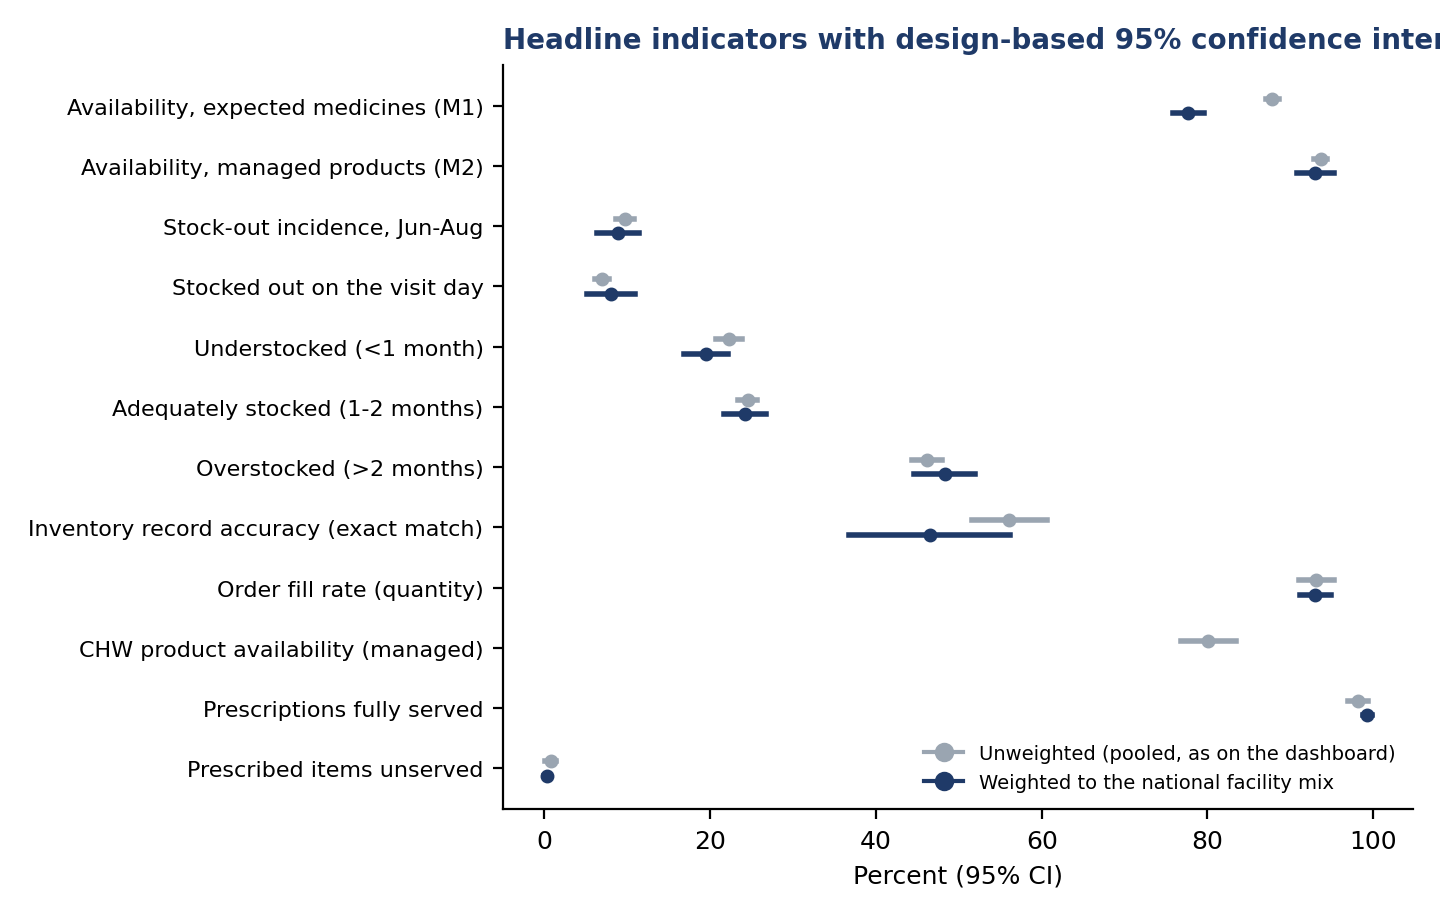
\includegraphics[width=0.94\linewidth]{fig_estimates.png}\caption*{\small Figure 1. Headline indicators with 95\% confidence intervals.}\end{figure}
\textbf{Interpretation.} The pooled figures on the dashboard are precise: the 95\% intervals for availability are about $\pm$1 point. Weighting changes the picture for expected-medicine availability (87.8\% pooled, 77.7\% weighted), because health posts make up most of Rwanda's facilities and stock fewer of the medicines the EML authorises for them; without health posts the weighted value (88.7\%) is close to the pooled one. Managed-product availability is robust to weighting. Record accuracy has a design effect of 19.1: accuracy is mostly a property of the facility, so its interval (51.6-60.6\%) is much wider than the 8,856 records would suggest, and its weighted value (46.5\%) is lower because health posts keep the least accurate records. The prescription indicators are very precise but, as noted on the dashboard, understate unmet need by design.

\subsection{Differences between groups}
{\footnotesize\setlength{\tabcolsep}{3pt}
\begin{longtable}{>{\raggedright\arraybackslash}p{0.279\linewidth}>{\raggedright\arraybackslash}p{0.279\linewidth}>{\raggedright\arraybackslash}p{0.279\linewidth}>{\raggedright\arraybackslash}p{0.133\linewidth}}
\rowcolor{navy}\textbf{\color{white}Level of care} & \textbf{\color{white}Managed availability \% (95\% CI)} & \textbf{\color{white}Stock-out incidence \% (95\% CI)} & \textbf{\color{white}Facilities} \\
\endhead
District hospital & 96.7 (95.1-98.4) & 5.6 (3.2-8.0) & 24 \\
\rowcolor{band}Health centre & 93.4 (92.6-94.3) & 10.3 (9.0-11.6) & 205 \\
Health post & 92.6 (88.6-96.5) & 8.1 (3.8-12.4) & 25 \\
\rowcolor{band}Level 2 teaching hospital & 91.9 (88.7-95.1) & 10.6 (5.6-15.5) & 10 \\
National referral hospital & 93.0 (92.4-93.7) & 14.0 (-1.0-28.9) & 2 \\
\end{longtable}}
{\footnotesize\setlength{\tabcolsep}{3pt}
\begin{longtable}{>{\raggedright\arraybackslash}p{0.279\linewidth}>{\raggedright\arraybackslash}p{0.279\linewidth}>{\raggedright\arraybackslash}p{0.279\linewidth}>{\raggedright\arraybackslash}p{0.133\linewidth}}
\rowcolor{navy}\textbf{\color{white}Management type} & \textbf{\color{white}Managed availability \% (95\% CI)} & \textbf{\color{white}Stock-out incidence \% (95\% CI)} & \textbf{\color{white}Facilities} \\
\endhead
Faith based facility based & 95.0 (93.8-96.3) & 7.9 (5.8-9.9) & 72 \\
\rowcolor{band}Government & 93.3 (92.4-94.2) & 10.4 (9.0-11.8) & 167 \\
PPP & 92.1 (88.4-95.8) & 8.7 (4.6-12.7) & 26 \\
\end{longtable}}
{\footnotesize\setlength{\tabcolsep}{3pt}
\begin{longtable}{>{\raggedright\arraybackslash}p{0.279\linewidth}>{\raggedright\arraybackslash}p{0.279\linewidth}>{\raggedright\arraybackslash}p{0.279\linewidth}>{\raggedright\arraybackslash}p{0.133\linewidth}}
\rowcolor{navy}\textbf{\color{white}Province} & \textbf{\color{white}Managed availability \% (95\% CI)} & \textbf{\color{white}Stock-out incidence \% (95\% CI)} & \textbf{\color{white}Facilities} \\
\endhead
East & 93.2 (91.8-94.6) & 11.2 (8.7-13.7) & 65 \\
\rowcolor{band}Kigali City & 94.8 (93.5-96.0) & 7.3 (5.3-9.3) & 26 \\
North & 93.1 (91.1-95.0) & 10.7 (8.4-13.1) & 50 \\
\rowcolor{band}South & 94.9 (93.6-96.2) & 8.1 (5.8-10.4) & 71 \\
West & 92.7 (90.8-94.6) & 9.9 (7.7-12.2) & 54 \\
\end{longtable}}
{\footnotesize\setlength{\tabcolsep}{3pt}
\begin{longtable}{>{\raggedright\arraybackslash}p{0.279\linewidth}>{\raggedright\arraybackslash}p{0.279\linewidth}>{\raggedright\arraybackslash}p{0.279\linewidth}>{\raggedright\arraybackslash}p{0.133\linewidth}}
\rowcolor{navy}\textbf{\color{white}Rms hub} & \textbf{\color{white}Managed availability \% (95\% CI)} & \textbf{\color{white}Stock-out incidence \% (95\% CI)} & \textbf{\color{white}Facilities} \\
\endhead
Huye HUB & 95.3 (93.9-96.7) & 8.6 (5.9-11.2) & 61 \\
\rowcolor{band}Karongi HUB & 92.8 (90.4-95.2) & 9.7 (6.7-12.8) & 35 \\
Kayonza HUB & 93.8 (92.3-95.4) & 10.2 (7.4-12.9) & 55 \\
\rowcolor{band}Kigali HUB & 92.4 (91.0-93.7) & 9.3 (7.5-11.2) & 66 \\
Musanze HUB & 93.8 (92.0-95.6) & 10.9 (8.6-13.2) & 49 \\
\end{longtable}}
\textbf{Interpretation.} Overlapping intervals mean many apparent differences on the dashboard are within sampling error. Of the 30 districts, 5 have managed availability significantly below the national value (Gicumbi, Ngoma, Gakenke, Bugesera, Rubavu) and 9 significantly above (Kicukiro, Gisagara, Nyanza, Huye, Muhanga, Nyamasheke, Musanze, Rwamagana, Burera); the remaining 16 cannot be distinguished from the national figure with 5-11 facilities each. District maps should be read with this in mind.

\subsection{Where the variation lies}
{\footnotesize\setlength{\tabcolsep}{3pt}
\begin{longtable}{>{\raggedright\arraybackslash}p{0.308\linewidth}>{\raggedright\arraybackslash}p{0.217\linewidth}>{\raggedright\arraybackslash}p{0.217\linewidth}>{\raggedright\arraybackslash}p{0.228\linewidth}}
\rowcolor{navy}\textbf{\color{white}Outcome} & \textbf{\color{white}Between facilities} & \textbf{\color{white}Between districts} & \textbf{\color{white}Within facility (residual)} \\
\endhead
Available on the visit day & 9.8\% & 3.3\% & 86.9\% \\
\rowcolor{band}Any stock-out day, Jun-Aug & 10.4\% & 6.5\% & 83.0\% \\
Exact record match & 50.0\% & 23.3\% & 26.7\% \\
\multicolumn{4}{p{0.97\linewidth}}{\scriptsize\itshape Variance partition from random-intercept logistic models (latent scale).}\\
\end{longtable}}
\textbf{Interpretation.} For availability and stock-outs, most variation is between medicines within the same facility; facilities and districts explain only 13.1\% and 16.9\%. Stock problems are therefore mostly medicine-specific, and national or programme-level supply actions matter as much as facility mentorship. Record accuracy is the opposite: 50.0\% of its variation is between facilities and 23.3\% between districts. A facility either keeps its records reconciled or it does not, which makes accuracy a natural target for facility-level QMIA mentorship.

\subsection{Determinants of availability (Model 1)}
{\footnotesize\setlength{\tabcolsep}{3pt}
\begin{longtable}{>{\raggedright\arraybackslash}p{0.571\linewidth}>{\raggedright\arraybackslash}p{0.251\linewidth}>{\raggedright\arraybackslash}p{0.148\linewidth}}
\rowcolor{navy}\textbf{\color{white}Factor} & \textbf{\color{white}Adjusted OR (95\% CI)} & \textbf{\color{white}p} \\
\endhead
Level: District hospital (ref. Health centre) & 3.29 (1.78-6.08) & $<$0.001 \\
\rowcolor{band}Level: Health post (ref. Health centre) & 1.70 (0.70-4.15) & 0.241 \\
Level: Referral / teaching (ref. Health centre) & 1.18 (0.66-2.11) & 0.569 \\
\rowcolor{band}Management: Faith-based (ref. Government) & 1.41 (1.03-1.92) & 0.030 \\
Management: PPP (ref. Government) & 0.49 (0.24-1.01) & 0.052 \\
\rowcolor{band}Province: East (ref. Kigali City) & 0.78 (0.55-1.11) & 0.172 \\
Province: North (ref. Kigali City) & 0.71 (0.48-1.07) & 0.103 \\
\rowcolor{band}Province: South (ref. Kigali City) & 0.92 (0.60-1.40) & 0.694 \\
Province: West (ref. Kigali City) & 0.60 (0.39-0.93) & 0.021 \\
\rowcolor{band}Programme: ARV (ref. Essential Medicines) & 0.67 (0.51-0.87) & 0.003 \\
Programme: Consumables (ref. Essential Medicines) & 1.53 (1.09-2.14) & 0.013 \\
\rowcolor{band}Programme: FP (ref. Essential Medicines) & 0.98 (0.74-1.30) & 0.882 \\
Programme: MCCH (ref. Essential Medicines) & 1.24 (0.85-1.82) & 0.264 \\
\rowcolor{band}Programme: Malaria (ref. Essential Medicines) & 13.89 (4.42-43.62) & $<$0.001 \\
Programme: TB (ref. Essential Medicines) & 0.81 (0.59-1.13) & 0.212 \\
\rowcolor{band}Setting: urban (ref. rural) & 1.02 (0.73-1.41) & 0.929 \\
Main digital system: Medisoft (ref. eLMIS) & 0.88 (0.56-1.38) & 0.576 \\
\rowcolor{band}Main digital system: OpenMRS (ref. eLMIS) & 0.60 (0.35-1.02) & 0.059 \\
Main digital system: Other / none (ref. eLMIS) & 0.91 (0.54-1.53) & 0.718 \\
\rowcolor{band}Main digital system: eBuzima (ref. eLMIS) & 1.00 (0.69-1.45) & 0.986 \\
Facility fill rate (per +10 points) & 0.99 (0.88-1.12) & 0.904 \\
\rowcolor{band}Facility record accuracy (per +10 points) & 0.97 (0.94-1.01) & 0.128 \\
\multicolumn{3}{p{0.97\linewidth}}{\scriptsize\itshape Outcome: managed medicine available on the visit day. n = 8,861 pairs, 265 facilities.}\\
\end{longtable}}
\begin{figure}[htbp]\centering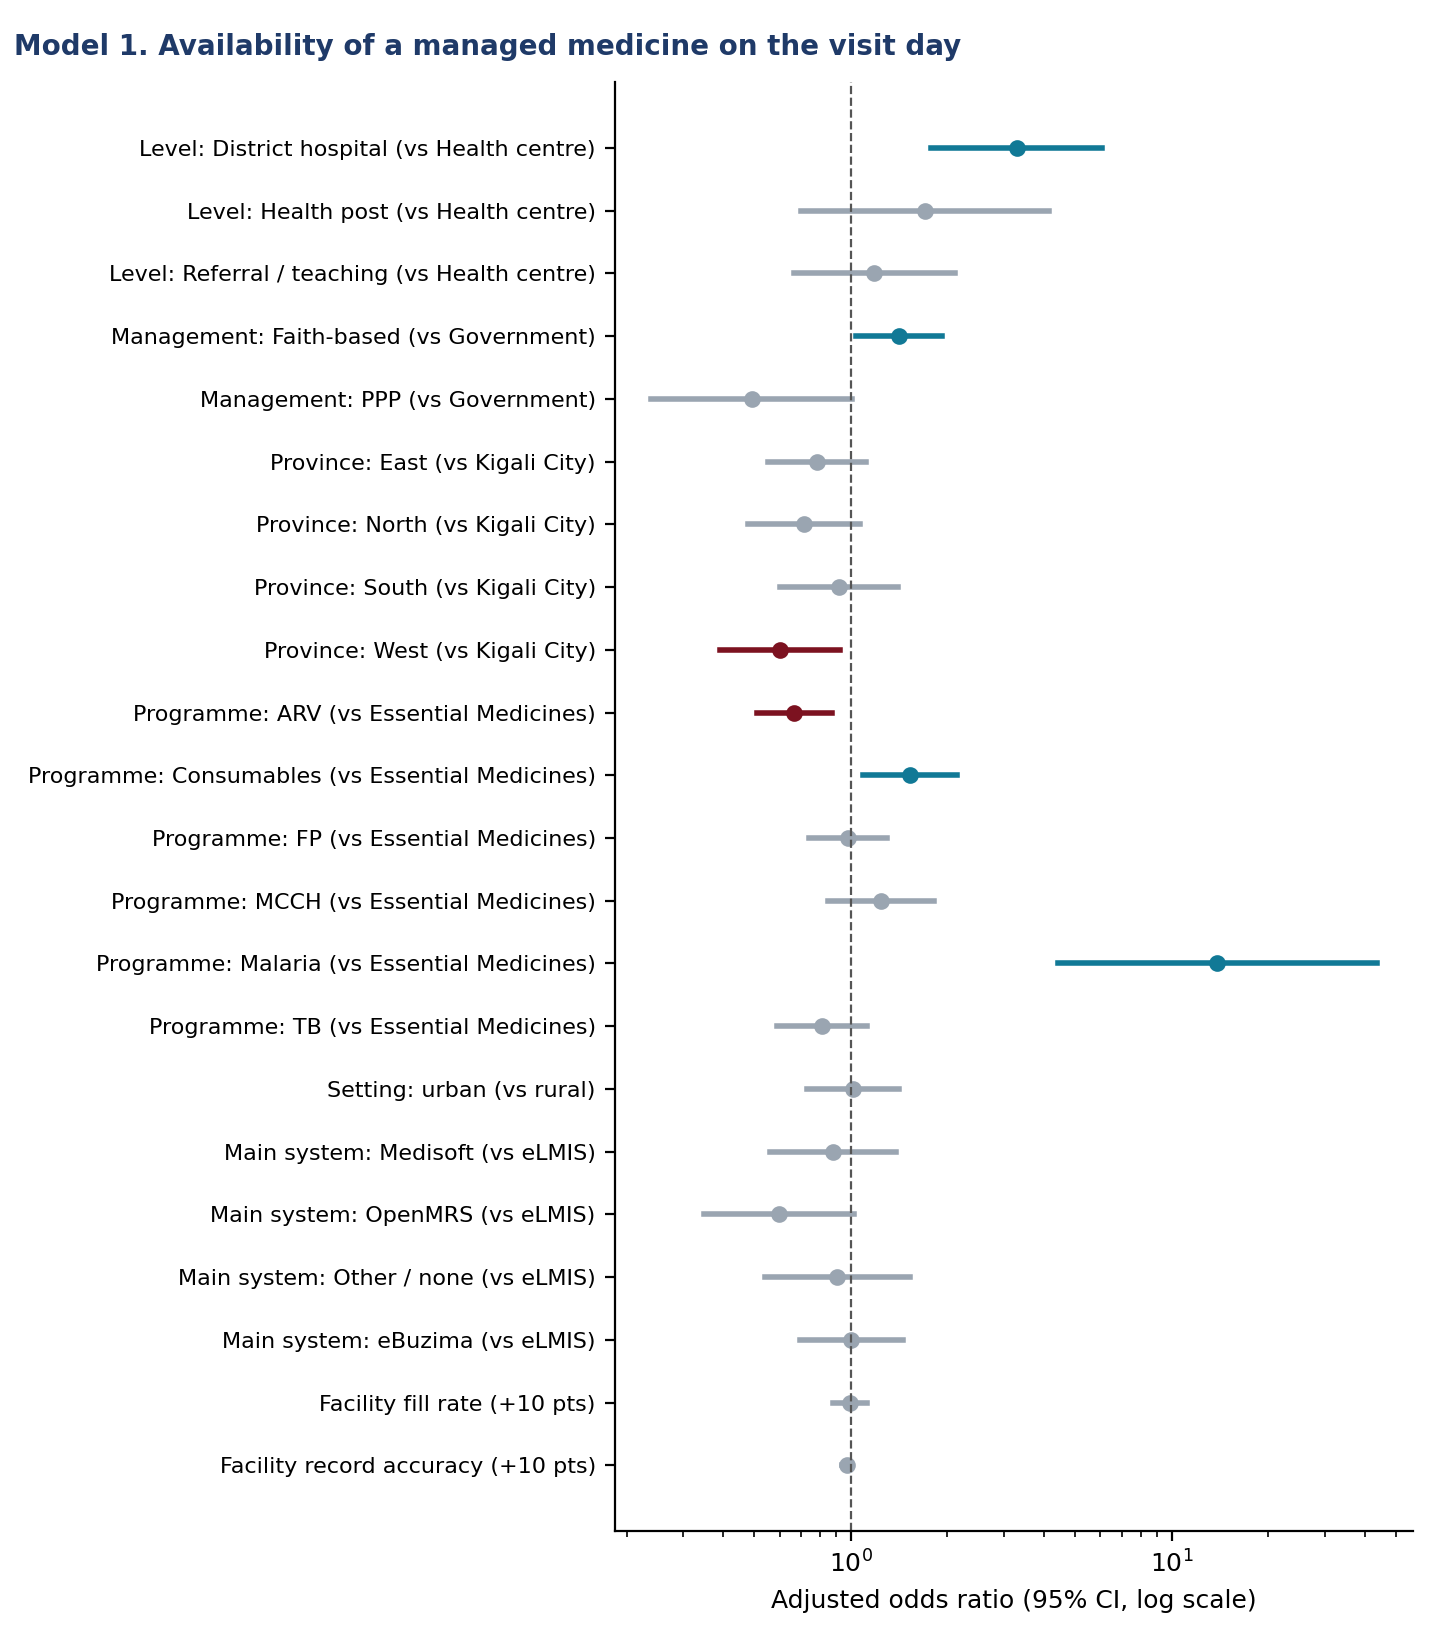
\includegraphics[width=0.76\linewidth]{fig_forest_availability.png}\caption*{\small Figure 2. Adjusted odds ratios for availability.}\end{figure}
\textbf{Interpretation.} With level, ownership, location, programme and system held constant, district hospitals are about three times as likely as health centres to have a managed medicine on the shelf (OR 3.29 (1.78-6.08)). Faith-based facilities do better than government ones (OR 1.41 (1.03-1.92)), as in Malawi [Mohan 2024]. The West is the only province significantly below Kigali City (OR 0.60 (0.39-0.93)). Among programmes, malaria commodities are almost always present (OR 13.89 (4.42-43.62)) and ARV products least (OR 0.67 (0.51-0.87)), consistent with the nationwide ARV stock-outs on the dashboard. Neither the facility's fill rate, its record accuracy, its digital system nor urban setting predicts availability once these are accounted for: availability is driven more by what is in the national pipeline for a given medicine than by facility traits.

\subsection{Determinants of stock-outs (Model 2)}
{\footnotesize\setlength{\tabcolsep}{3pt}
\begin{longtable}{>{\raggedright\arraybackslash}p{0.571\linewidth}>{\raggedright\arraybackslash}p{0.251\linewidth}>{\raggedright\arraybackslash}p{0.148\linewidth}}
\rowcolor{navy}\textbf{\color{white}Factor} & \textbf{\color{white}Adjusted OR (95\% CI)} & \textbf{\color{white}p} \\
\endhead
Level: District hospital (ref. Health centre) & 0.64 (0.39-1.05) & 0.080 \\
\rowcolor{band}Level: Health post (ref. Health centre) & 0.53 (0.28-1.02) & 0.059 \\
Level: Referral / teaching (ref. Health centre) & 1.43 (0.78-2.61) & 0.251 \\
\rowcolor{band}Management: Faith-based (ref. Government) & 0.76 (0.55-1.04) & 0.090 \\
Management: PPP (ref. Government) & 1.28 (0.80-2.06) & 0.304 \\
\rowcolor{band}Province: East (ref. Kigali City) & 1.69 (1.06-2.68) & 0.027 \\
Province: North (ref. Kigali City) & 1.54 (0.99-2.39) & 0.056 \\
\rowcolor{band}Province: South (ref. Kigali City) & 1.20 (0.71-2.02) & 0.492 \\
Province: West (ref. Kigali City) & 1.52 (0.97-2.38) & 0.069 \\
\rowcolor{band}Programme: ARV (ref. Essential Medicines) & 0.49 (0.38-0.62) & $<$0.001 \\
Programme: Consumables (ref. Essential Medicines) & 0.38 (0.29-0.50) & $<$0.001 \\
\rowcolor{band}Programme: FP (ref. Essential Medicines) & 0.26 (0.19-0.35) & $<$0.001 \\
Programme: MCCH (ref. Essential Medicines) & 0.25 (0.19-0.34) & $<$0.001 \\
\rowcolor{band}Programme: Malaria (ref. Essential Medicines) & 0.06 (0.04-0.11) & $<$0.001 \\
Programme: TB (ref. Essential Medicines) & 0.36 (0.26-0.50) & $<$0.001 \\
\rowcolor{band}Setting: urban (ref. rural) & 1.05 (0.74-1.50) & 0.766 \\
log(AMC + 1) & 0.79 (0.75-0.82) & $<$0.001 \\
\rowcolor{band}Erratic consumption (CV $\geq$ 50\%) & 1.33 (1.13-1.55) & $<$0.001 \\
Facility fill rate (per +10 points) & 0.98 (0.86-1.11) & 0.713 \\
\rowcolor{band}Facility record accuracy (per +10 points) & 1.01 (0.97-1.04) & 0.730 \\
\multicolumn{3}{p{0.97\linewidth}}{\scriptsize\itshape Outcome: any stock-out day June-August. n = 9,590 pairs.}\\
\end{longtable}}
\begin{figure}[htbp]\centering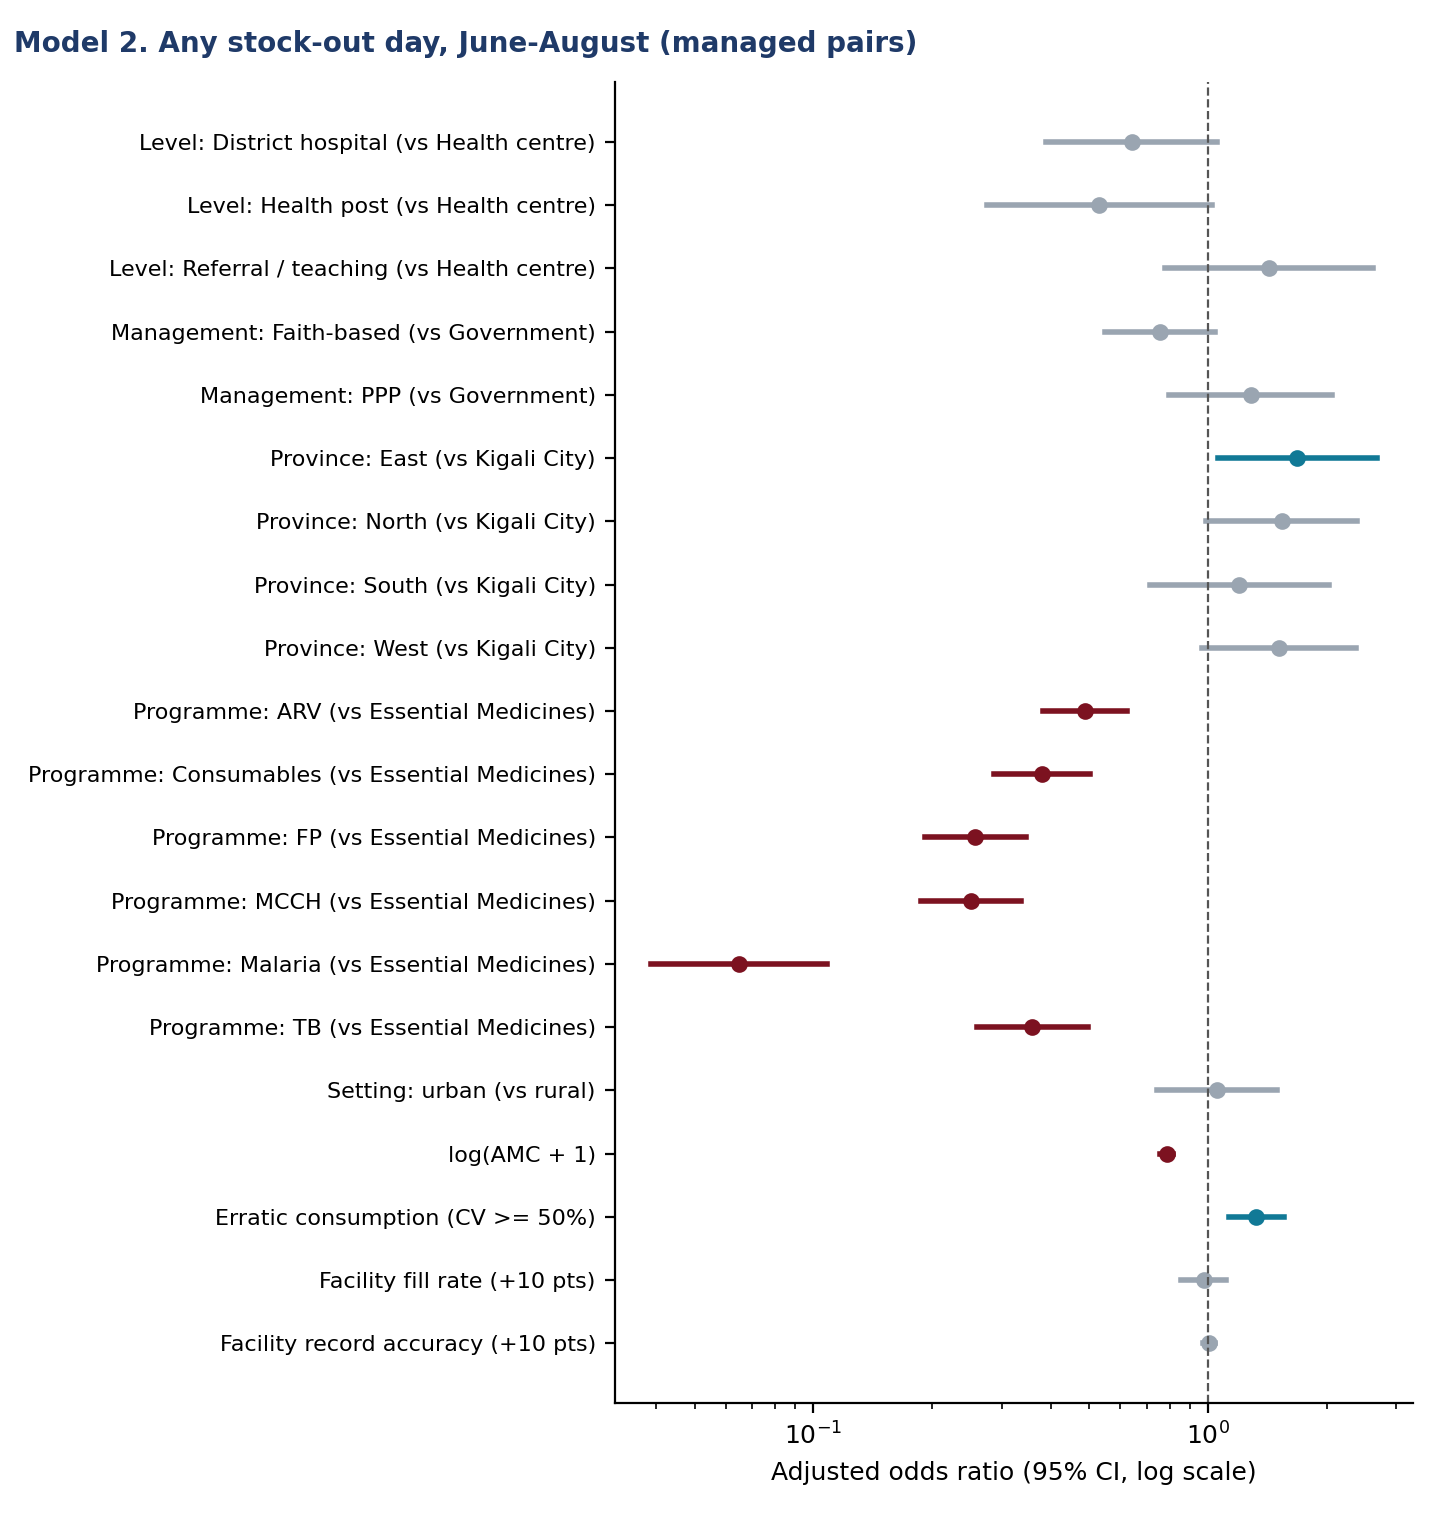
\includegraphics[width=0.76\linewidth]{fig_forest_stockout.png}\caption*{\small Figure 3. Adjusted odds ratios for stock-out incidence.}\end{figure}
\textbf{Interpretation.} Every vertical programme has far lower odds of a stock-out than essential medicines (OR 0.06 for malaria to 0.49 for ARV). This reflects separate, programme-managed pipelines with push distribution and larger buffer stocks, which is also why these programmes are the most overstocked. Higher-volume medicines are less often out (OR 0.79 (0.75-0.82) per unit log AMC), and medicines with erratic month-to-month consumption more often (OR 1.33 (1.13-1.55)): an average-based order quantity fails exactly where demand is irregular. Eastern facilities have higher odds than Kigali City (OR 1.69 (1.06-2.68)).

\subsection{Does order fulfilment drive stock-outs? (Model 4)}
{\footnotesize\setlength{\tabcolsep}{3pt}
\begin{longtable}{>{\raggedright\arraybackslash}p{0.399\linewidth}>{\raggedright\arraybackslash}p{0.228\linewidth}>{\raggedright\arraybackslash}p{0.342\linewidth}}
\rowcolor{navy}\textbf{\color{white}Order outcome this month} & \textbf{\color{white}Pair-months} & \textbf{\color{white}Stocked out next month} \\
\endhead
Delivered in full & 6,848 & 2.9\% \\
\rowcolor{band}No request & 11,669 & 7.9\% \\
Partly delivered & 300 & 4.3\% \\
\rowcolor{band}Requested, nothing delivered & 363 & 36.9\% \\
\end{longtable}}
{\footnotesize\setlength{\tabcolsep}{3pt}
\begin{longtable}{>{\raggedright\arraybackslash}p{0.571\linewidth}>{\raggedright\arraybackslash}p{0.251\linewidth}>{\raggedright\arraybackslash}p{0.148\linewidth}}
\rowcolor{navy}\textbf{\color{white}Factor} & \textbf{\color{white}Adjusted OR (95\% CI)} & \textbf{\color{white}p} \\
\endhead
Order outcome this month: No request (ref. Delivered in full) & 2.64 (1.94-3.61) & $<$0.001 \\
\rowcolor{band}Order outcome this month: Partly delivered (ref. Delivered in full) & 0.54 (0.23-1.28) & 0.165 \\
Order outcome this month: Requested, nothing delivered (ref. Delivered in full) & 7.62 (4.57-12.70) & $<$0.001 \\
\rowcolor{band}Month: August & 0.93 (0.77-1.14) & 0.491 \\
Level: District hospital (ref. Health centre) & 0.69 (0.47-1.00) & 0.049 \\
\rowcolor{band}Level: Health post (ref. Health centre) & 0.73 (0.47-1.12) & 0.151 \\
Level: Referral / teaching (ref. Health centre) & 1.67 (1.06-2.63) & 0.027 \\
\rowcolor{band}Programme: ARV (ref. Essential Medicines) & 0.68 (0.50-0.92) & 0.013 \\
Programme: Consumables (ref. Essential Medicines) & 0.59 (0.44-0.79) & $<$0.001 \\
\rowcolor{band}Programme: FP (ref. Essential Medicines) & 0.50 (0.38-0.64) & $<$0.001 \\
Programme: MCCH (ref. Essential Medicines) & 0.46 (0.34-0.61) & $<$0.001 \\
\rowcolor{band}Programme: Malaria (ref. Essential Medicines) & 0.12 (0.08-0.17) & $<$0.001 \\
Programme: TB (ref. Essential Medicines) & 0.46 (0.34-0.62) & $<$0.001 \\
\rowcolor{band}Stocked out this month & 117.39 (91.96-149.85) & $<$0.001 \\
log(AMC + 1) & 0.89 (0.86-0.93) & $<$0.001 \\
\multicolumn{3}{p{0.97\linewidth}}{\scriptsize\itshape Outcome: any stock-out day in month t+1. n = 19,180 pair-months.}\\
\end{longtable}}
\begin{figure}[htbp]\centering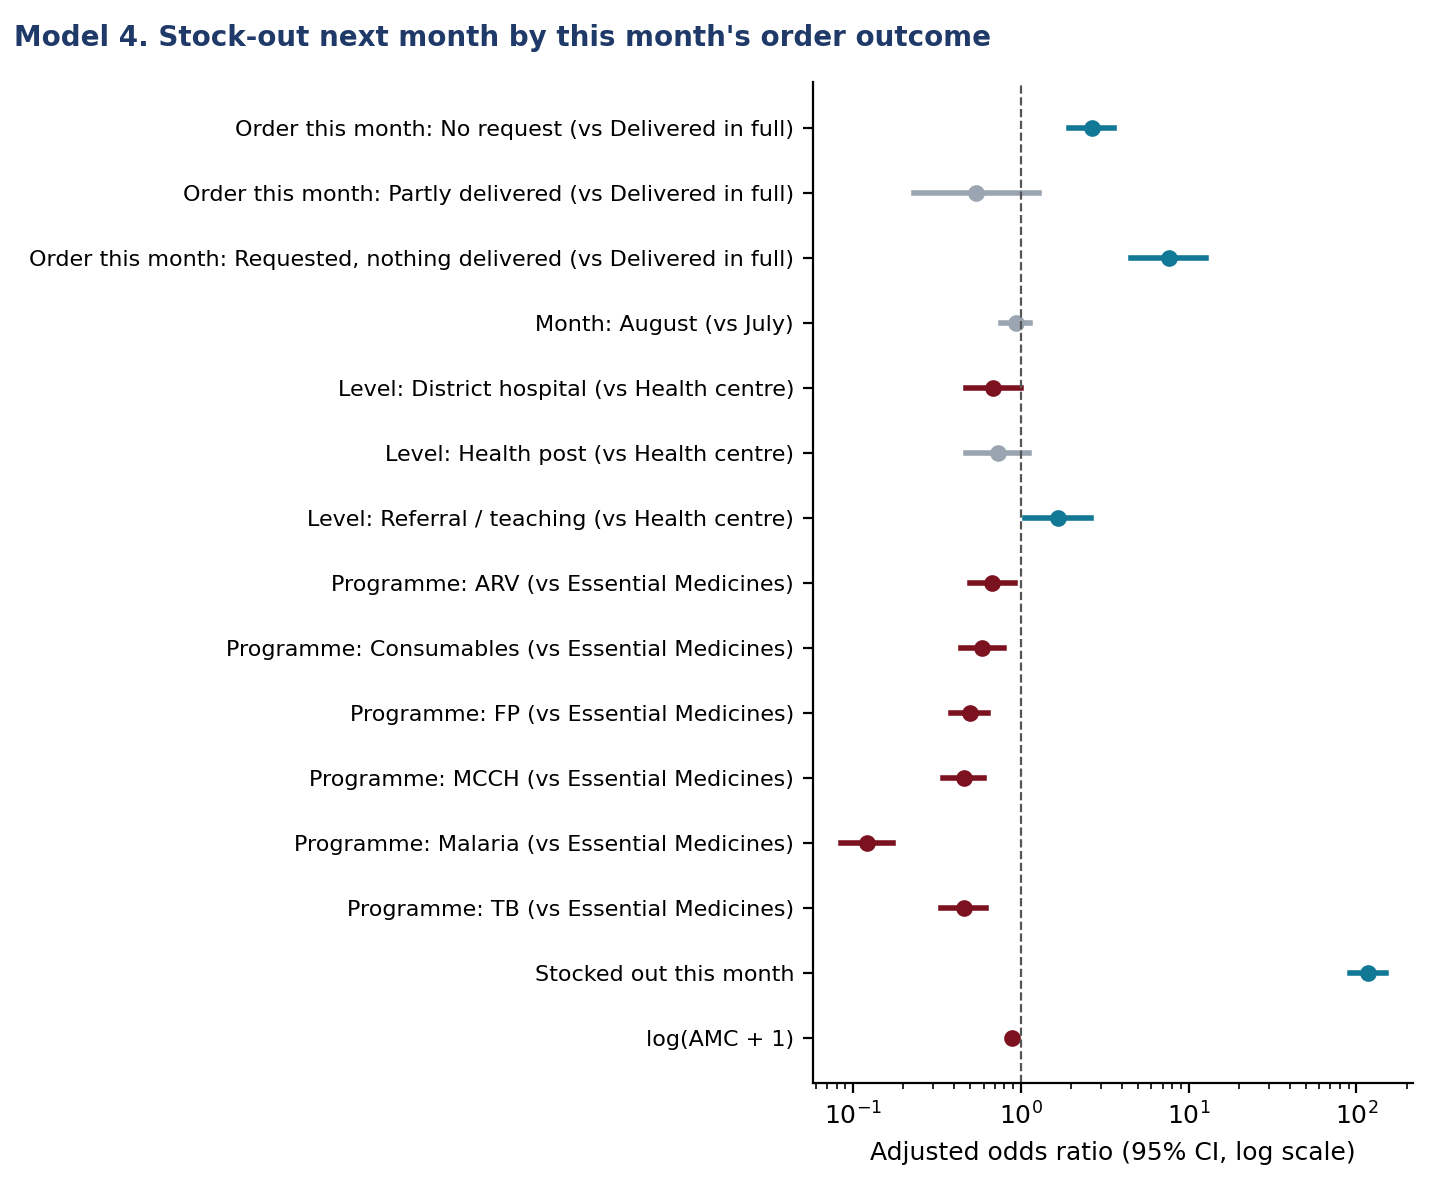
\includegraphics[width=0.76\linewidth]{fig_forest_lag.png}\caption*{\small Figure 4. Next-month stock-out by this month's order outcome.}\end{figure}
\textbf{Interpretation.} This is the clearest causal signal in the data, because the exposure precedes the outcome. When a facility requested a medicine and received nothing, 36.9\% of those pairs were out the next month, and the adjusted odds were 7.6 times those after a full delivery, even after accounting for whether the medicine was already out. Partial deliveries carried no excess risk, so the problem is orders that go entirely unfilled, not quantities trimmed. Not requesting at all also raised the odds (OR 2.64 (1.94-3.61)), pointing to missed or late orders at the facility. Being out this month was by far the strongest predictor (OR 117): once a stock-out starts it tends to last. Together these support two actions: RMS should flag and expedite nil-filled orders, and facilities should not skip a requisition cycle.

\subsection{Inventory record accuracy (Model 3)}
{\footnotesize\setlength{\tabcolsep}{3pt}
\begin{longtable}{>{\raggedright\arraybackslash}p{0.571\linewidth}>{\raggedright\arraybackslash}p{0.251\linewidth}>{\raggedright\arraybackslash}p{0.148\linewidth}}
\rowcolor{navy}\textbf{\color{white}Factor} & \textbf{\color{white}Adjusted OR (95\% CI)} & \textbf{\color{white}p} \\
\endhead
Digital system: Medisoft (ref. eLMIS) & 0.36 (0.15-0.83) & 0.017 \\
\rowcolor{band}Digital system: OpenMRS (ref. eLMIS) & 0.48 (0.15-1.54) & 0.218 \\
Digital system: Other (ref. eLMIS) & 0.50 (0.19-1.34) & 0.168 \\
\rowcolor{band}Digital system: eBuzima (ref. eLMIS) & 0.26 (0.15-0.46) & $<$0.001 \\
Level: District hospital (ref. Health centre) & 5.91 (2.21-15.84) & $<$0.001 \\
\rowcolor{band}Level: Health post (ref. Health centre) & 2.36 (0.50-11.18) & 0.279 \\
Level: Referral / teaching (ref. Health centre) & 2.64 (0.59-11.86) & 0.207 \\
\rowcolor{band}Management: Faith-based (ref. Government) & 1.00 (0.61-1.63) & 0.994 \\
Management: PPP (ref. Government) & 0.16 (0.04-0.73) & 0.018 \\
\rowcolor{band}Province: East (ref. Kigali City) & 2.00 (1.08-3.71) & 0.027 \\
Province: North (ref. Kigali City) & 1.63 (0.82-3.26) & 0.163 \\
\rowcolor{band}Province: South (ref. Kigali City) & 0.74 (0.36-1.53) & 0.412 \\
Province: West (ref. Kigali City) & 1.02 (0.45-2.32) & 0.956 \\
\rowcolor{band}Programme: ARV (ref. Essential Medicines) & 1.17 (0.96-1.41) & 0.115 \\
Programme: Consumables (ref. Essential Medicines) & 0.82 (0.72-0.94) & 0.004 \\
\rowcolor{band}Programme: FP (ref. Essential Medicines) & 0.87 (0.72-1.05) & 0.155 \\
Programme: MCCH (ref. Essential Medicines) & 1.13 (0.93-1.38) & 0.212 \\
\rowcolor{band}Programme: Malaria (ref. Essential Medicines) & 1.01 (0.85-1.21) & 0.900 \\
Programme: TB (ref. Essential Medicines) & 0.98 (0.80-1.20) & 0.827 \\
\multicolumn{3}{p{0.97\linewidth}}{\scriptsize\itshape Outcome: physical count equals system count. n = 8,822 records.}\\
\end{longtable}}
\begin{figure}[htbp]\centering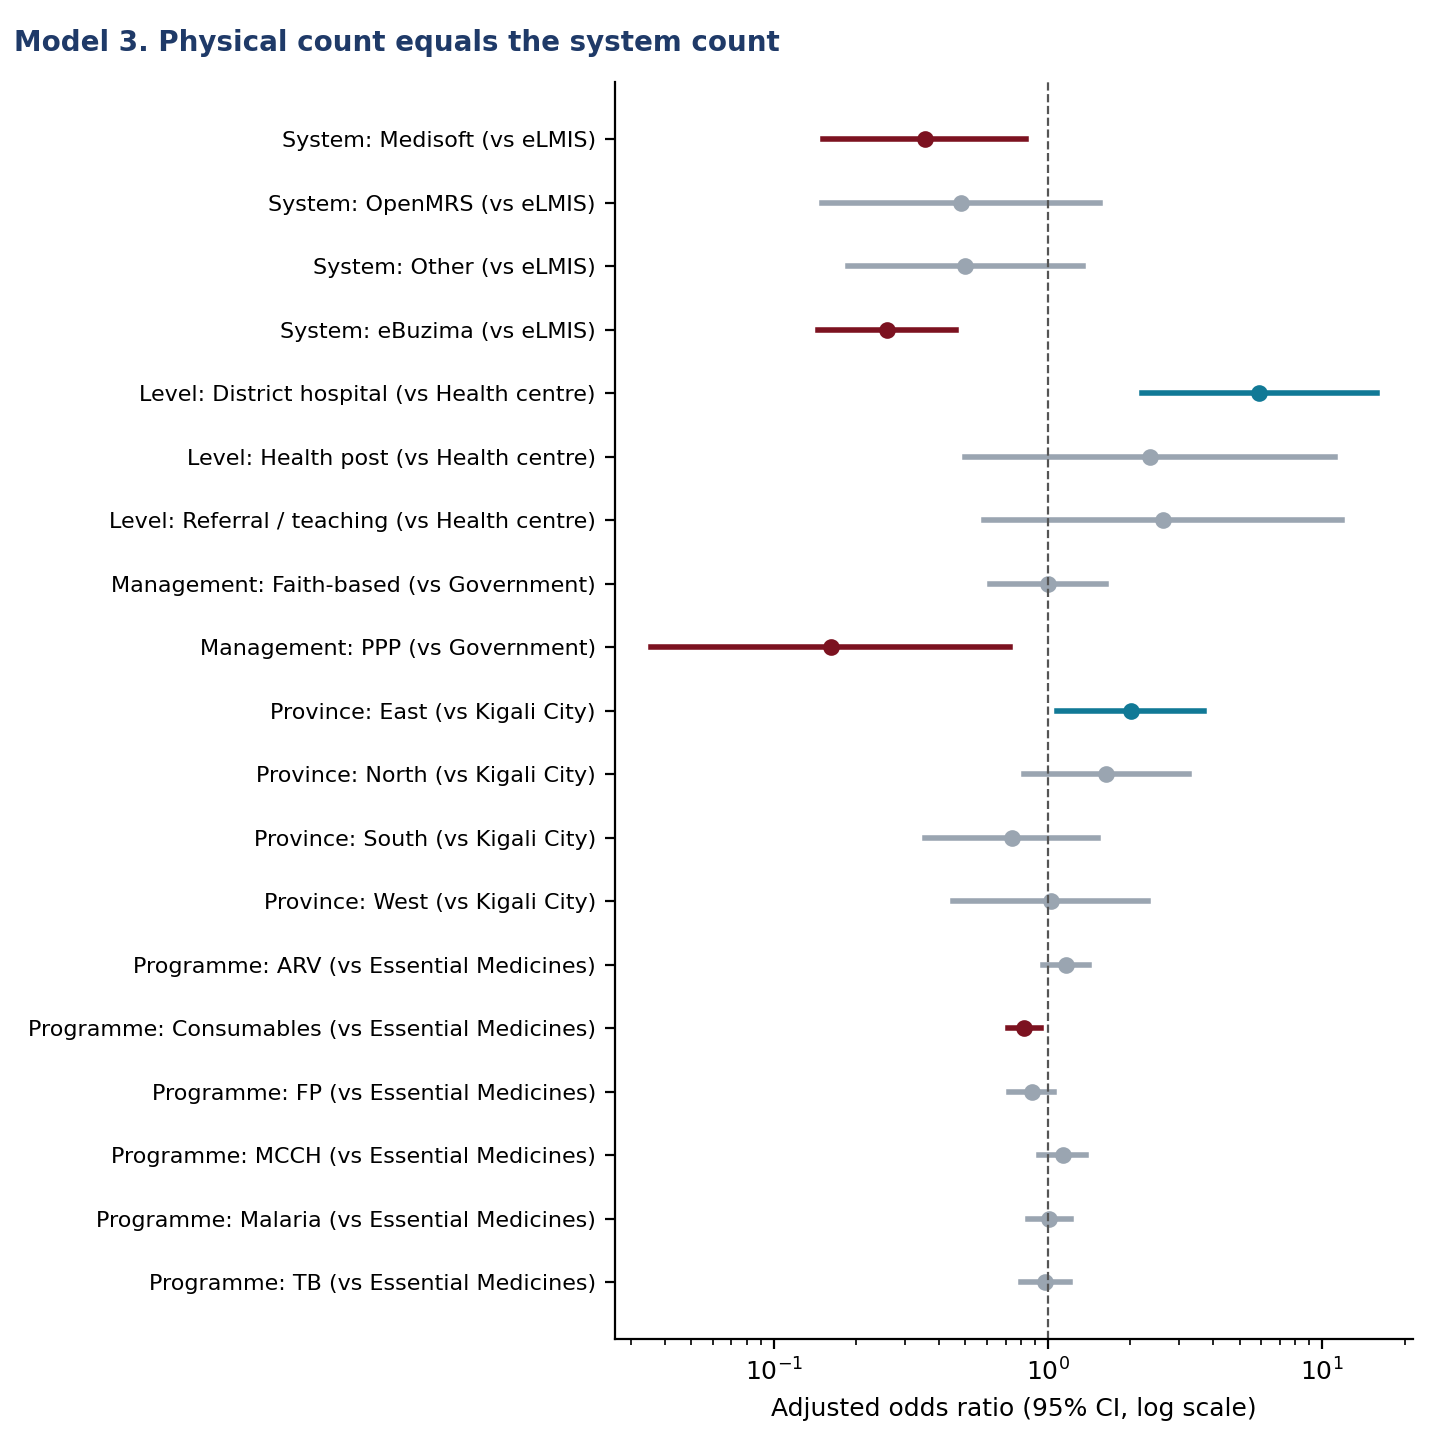
\includegraphics[width=0.76\linewidth]{fig_forest_accuracy.png}\caption*{\small Figure 5. Adjusted odds ratios for exact record match.}\end{figure}
\textbf{Interpretation.} Records kept in eBuzima matched the shelf far less often than eLMIS records (OR 0.26 (0.15-0.46)), as did Medisoft (OR 0.36 (0.15-0.83)), after level and location are held constant. eBuzima is a point-of-care system whose stock module depends on dispensing being recorded for every patient, which the data-collector feedback says is often not done. District hospitals are much more accurate than health centres (OR 5.91 (2.21-15.84)) and PPP facilities much less (OR 0.16 (0.04-0.73)). The Rwandan QMIA reached 85\% accuracy by 2019 [Kigenza 2023]. Definitions may differ, but today's 56\% suggests that some of that gain has been lost; the eBuzima result points to the transition of health centres to point-of-care systems as one likely reason.

\subsection{Prescribing quality and unserved prescriptions}
{\footnotesize\setlength{\tabcolsep}{3pt}
\begin{longtable}{>{\raggedright\arraybackslash}p{0.297\linewidth}>{\raggedright\arraybackslash}p{0.240\linewidth}>{\raggedright\arraybackslash}p{0.171\linewidth}>{\raggedright\arraybackslash}p{0.262\linewidth}}
\rowcolor{navy}\textbf{\color{white}WHO indicator} & \textbf{\color{white}Estimate (95\% CI)} & \textbf{\color{white}WHO reference} & \textbf{\color{white}Africa median [Ofori-Asenso 2016]} \\
\endhead
Medicines per encounter & 2.25 (2.14-2.36) & $<$ 2 (1.6-1.8) & 3.1 \\
\rowcolor{band}Generic (INN) prescribing & 97.2\% (95.3-99.1) & 100\% & 68.0\% \\
Encounters with an antibiotic & 49.5\% (44.9-54.2) & $<$ 30\% & 46.8\% \\
\rowcolor{band}Encounters with an injection & 8.8\% (6.2-11.5) & $<$ 20\% & 25.0\% \\
Medicines from the EML & 95.4\% (90.3-100.0) & 100\% & 88.0\% \\
\multicolumn{4}{p{0.97\linewidth}}{\scriptsize\itshape Weighted by level; facility-clustered 95\% CI.}\\
\end{longtable}}
{\footnotesize\setlength{\tabcolsep}{3pt}
\begin{longtable}{>{\raggedright\arraybackslash}p{0.297\linewidth}>{\raggedright\arraybackslash}p{0.160\linewidth}>{\raggedright\arraybackslash}p{0.183\linewidth}>{\raggedright\arraybackslash}p{0.165\linewidth}>{\raggedright\arraybackslash}p{0.165\linewidth}}
\rowcolor{navy}\textbf{\color{white}Level} & \textbf{\color{white}Prescriptions} & \textbf{\color{white}Medicines / encounter} & \textbf{\color{white}\% antibiotic} & \textbf{\color{white}\% injection} \\
\endhead
District hospital & 739 & 2.52 & 36.9 & 30.0 \\
\rowcolor{band}Health centre & 4384 & 2.30 & 50.5 & 9.2 \\
Health post & 495 & 2.20 & 50.1 & 7.3 \\
\rowcolor{band}Level 2 teaching hospital & 318 & 2.46 & 34.3 & 31.4 \\
National referral hospital & 70 & 3.76 & 15.7 & 25.7 \\
\end{longtable}}
\begin{figure}[htbp]\centering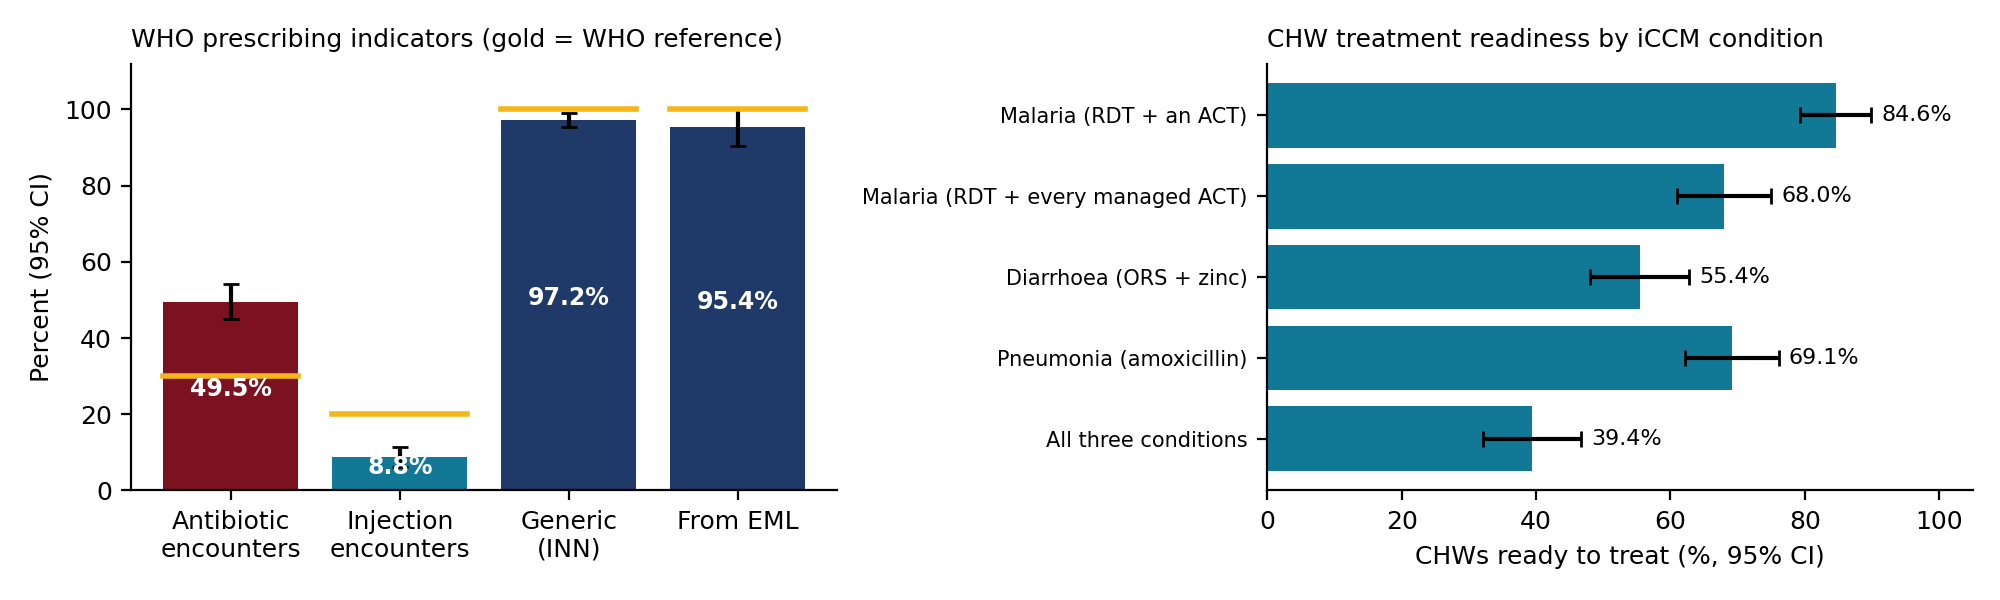
\includegraphics[width=0.94\linewidth]{fig_who_iccm.png}\caption*{\small Figure 6. WHO prescribing indicators (left) and CHW readiness by iCCM condition (right).}\end{figure}
{\footnotesize\setlength{\tabcolsep}{3pt}
\begin{longtable}{>{\raggedright\arraybackslash}p{0.456\linewidth}>{\raggedright\arraybackslash}p{0.257\linewidth}>{\raggedright\arraybackslash}p{0.257\linewidth}}
\rowcolor{navy}\textbf{\color{white}Factor} & \textbf{\color{white}Unserved: OR (95\% CI)} & \textbf{\color{white}Antibiotic: OR (95\% CI)} \\
\endhead
Prescriber: General practitioner (ref. Nurse) & 0.98 (0.20-4.88) & 2.18 (1.27-3.73) \\
\rowcolor{band}Prescriber: Other (ref. Nurse) & 3.23 (0.97-10.74) & 1.63 (0.99-2.67) \\
Prescriber: Specialist (ref. Nurse) & 10.16 (1.33-77.34) & 0.80 (0.28-2.31) \\
\rowcolor{band}Level: District hospital (ref. Primary care (HC/HP)) & 1.10 (0.26-4.67) & 0.25 (0.15-0.41) \\
Level: Referral / teaching (ref. Primary care (HC/HP)) & 2.14 (0.38-11.92) & 0.18 (0.10-0.34) \\
\rowcolor{band}Medicines on the prescription (per +1) & 1.34 (1.15-1.55) & 2.08 (1.88-2.31) \\
\multicolumn{3}{p{0.97\linewidth}}{\scriptsize\itshape Models 5 and 6. Outcomes: any unserved item; any antibiotic. Reference: nurse, primary care.}\\
\end{longtable}}
\textbf{Interpretation.} Prescribing in Rwanda compares well with the African median on generic names, EML adherence, polypharmacy and injections. Antibiotic use is the exception: 49.5\% of encounters, about the African median and well above the 30\% reference. It is concentrated in primary care (about half of health-centre and health-post encounters, against about a third in hospitals), and general practitioners prescribe antibiotics more often than nurses once the number of medicines is held constant (OR 2.18 (1.27-3.73)). This is a priority for antimicrobial stewardship. Unserved prescriptions are rare, but a specialist's prescription is far more likely to include an unavailable item (OR 10.16 (1.33-77.34)), as is a longer prescription (OR 1.34 (1.15-1.55) per medicine). This matches the referral-hospital gaps on the dashboard: specialist prescribing reaches beyond what the pharmacy stocks.

\subsection{Community level}
{\footnotesize\setlength{\tabcolsep}{3pt}
\begin{longtable}{>{\raggedright\arraybackslash}p{0.514\linewidth}>{\raggedright\arraybackslash}p{0.456\linewidth}}
\rowcolor{navy}\textbf{\color{white}Condition} & \textbf{\color{white}CHWs ready (95\% CI)} \\
\endhead
Malaria (RDT + an ACT) & 84.6\% (79.3-89.9) \\
\rowcolor{band}Malaria (RDT + every managed ACT) & 68.0\% (61.0-75.0) \\
Diarrhoea (ORS + zinc) & 55.4\% (48.1-62.8) \\
\rowcolor{band}Pneumonia (amoxicillin) & 69.1\% (62.2-76.1) \\
All three conditions & 39.4\% (32.1-46.7) \\
\end{longtable}}
{\footnotesize\setlength{\tabcolsep}{3pt}
\begin{longtable}{>{\raggedright\arraybackslash}p{0.240\linewidth}>{\raggedright\arraybackslash}p{0.183\linewidth}>{\raggedright\arraybackslash}p{0.183\linewidth}>{\raggedright\arraybackslash}p{0.183\linewidth}>{\raggedright\arraybackslash}p{0.183\linewidth}}
\rowcolor{navy}\textbf{\color{white}Province} & \textbf{\color{white}Malaria} & \textbf{\color{white}Diarrhoea} & \textbf{\color{white}Pneumonia} & \textbf{\color{white}All three} \\
\endhead
East & 87.0 & 45.7 & 73.9 & 34.8 \\
\rowcolor{band}Kigali City & 86.7 & 40.0 & 33.3 & 13.3 \\
North & 67.6 & 50.0 & 64.7 & 26.5 \\
\rowcolor{band}South & 93.9 & 61.2 & 75.5 & 51.0 \\
West & 83.9 & 74.2 & 74.2 & 54.8 \\
\multicolumn{5}{p{0.97\linewidth}}{\scriptsize\itshape Percent of CHWs ready.}\\
\end{longtable}}
{\footnotesize\setlength{\tabcolsep}{3pt}
\begin{longtable}{>{\raggedright\arraybackslash}p{0.285\linewidth}>{\raggedright\arraybackslash}p{0.103\linewidth}>{\raggedright\arraybackslash}p{0.148\linewidth}>{\raggedright\arraybackslash}p{0.171\linewidth}>{\raggedright\arraybackslash}p{0.160\linewidth}>{\raggedright\arraybackslash}p{0.103\linewidth}}
\rowcolor{navy}\textbf{\color{white}Product (molecule)} & \textbf{\color{white}Pairs} & \textbf{\color{white}CHW available} & \textbf{\color{white}Health centre available} & \textbf{\color{white}CHW out, HC has it} & \textbf{\color{white}McNemar p} \\
\endhead
arte & 52 & 98.1\% & 100.0\% & 1 & 1.000 \\
\rowcolor{band}dihydroartemisinin piperaquine & 57 & 87.7\% & 100.0\% & 7 & 0.016 \\
Malaria RDT & 170 & 94.1\% & 100.0\% & 10 & 0.002 \\
\rowcolor{band}pyronaridine artesunate & 56 & 89.3\% & 100.0\% & 6 & 0.031 \\
\multicolumn{6}{p{0.97\linewidth}}{\scriptsize\itshape CHW paired with the supervising health centre on the same molecule.}\\
\end{longtable}}
\textbf{Interpretation.} Treatment readiness is lower than product availability suggests: only 39.4\% of CHWs could treat malaria, diarrhoea and pneumonia on the visit day, below the 49\% SC4CCM baseline for Rwanda [Chandani 2014] although the product lists differ. Diarrhoea is the weakest condition because ORS and zinc must both be present. Kigali City has the lowest readiness, largely because of amoxicillin. In all 335 CHW-health centre pairs, the health centre had the product whenever the CHW did, and in every one of the 24 discordant pairs the CHW was out while the health centre had stock (exact p $<$0.001). The community gap is therefore one of resupply from the health centre to the CHW, which also matches the Bugesera finding that CHWs walk and pay to collect stock [Gakinahe 2024].

\subsection{Geography}
{\footnotesize\setlength{\tabcolsep}{3pt}
\begin{longtable}{>{\raggedright\arraybackslash}p{0.342\linewidth}>{\raggedright\arraybackslash}p{0.171\linewidth}>{\raggedright\arraybackslash}p{0.257\linewidth}>{\raggedright\arraybackslash}p{0.200\linewidth}}
\rowcolor{navy}\textbf{\color{white}District indicator} & \textbf{\color{white}Moran's I} & \textbf{\color{white}Expected under no clustering} & \textbf{\color{white}Permutation p} \\
\endhead
M2 availability & -0.092 & -0.034 & 0.668 \\
\rowcolor{band}M1 availability & -0.078 & -0.034 & 0.633 \\
Stock-out incidence & -0.179 & -0.034 & 0.924 \\
\rowcolor{band}Record accuracy & -0.072 & -0.034 & 0.596 \\
CHW availability & 0.152 & -0.036 & 0.050 \\
\end{longtable}}
\textbf{Interpretation.} Neighbouring districts are no more alike than distant ones for availability, stock-outs or record accuracy; weak districts are scattered rather than forming a region. CHW availability shows weak positive clustering (p about 0.05), consistent with zone-wide antimalarial allocation. In practice this means support should be allocated facility by facility rather than to a whole region.

\subsection{Facility typology}
{\footnotesize\setlength{\tabcolsep}{3pt}
\begin{longtable}{>{\raggedright\arraybackslash}p{0.262\linewidth}>{\raggedright\arraybackslash}p{0.103\linewidth}>{\raggedright\arraybackslash}p{0.103\linewidth}>{\raggedright\arraybackslash}p{0.097\linewidth}>{\raggedright\arraybackslash}p{0.097\linewidth}>{\raggedright\arraybackslash}p{0.097\linewidth}>{\raggedright\arraybackslash}p{0.103\linewidth}>{\raggedright\arraybackslash}p{0.108\linewidth}}
\rowcolor{navy}\textbf{\color{white}Profile} & \textbf{\color{white}Facilities} & \textbf{\color{white}Availability} & \textbf{\color{white}Stock-out} & \textbf{\color{white}Accuracy} & \textbf{\color{white}Fill rate} & \textbf{\color{white}Overstock} & \textbf{\color{white}Understock} \\
\endhead
1. Well supplied but overstocked & 92 & 96.8 & 5.7 & 55.6 & 96.1 & 62.4 & 10.1 \\
\rowcolor{band}2. Weak resupply and weak records & 35 & 93.0 & 10.3 & 40.4 & 77.1 & 46.8 & 22.8 \\
3. Frequent stock-outs & 54 & 85.6 & 21.9 & 59.9 & 96.5 & 34.8 & 25.7 \\
\rowcolor{band}4. Lean stock, often understocked & 85 & 95.9 & 5.5 & 55.2 & 97.1 & 37.0 & 31.8 \\
\multicolumn{8}{p{0.97\linewidth}}{\scriptsize\itshape Cluster means, percent. The facility list is in results/facility\_typology.csv.}\\
\end{longtable}}
\begin{figure}[htbp]\centering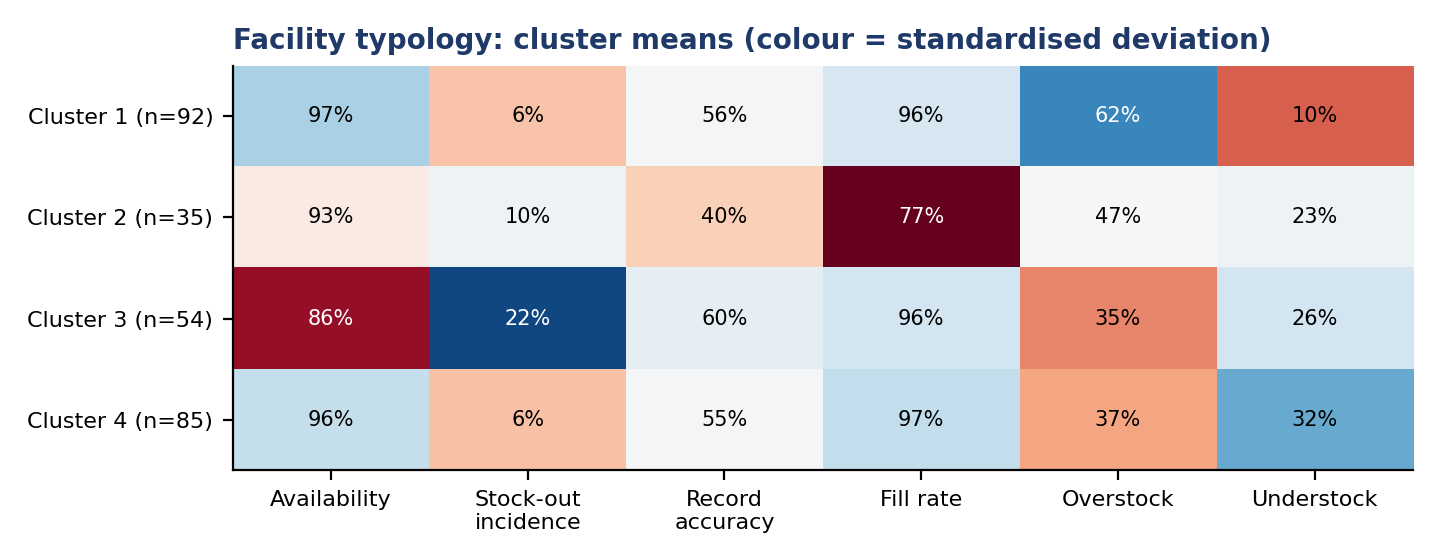
\includegraphics[width=0.88\linewidth]{fig_typology.png}\caption*{\small Figure 7. Facility profiles from k-means clustering.}\end{figure}
\textbf{Interpretation.} The profiles separate problems that need different responses. \textbf{Frequent stock-outs} facilities have the lowest availability despite normal fill rates, pointing to under-ordering and quantification. \textbf{Weak resupply and weak records} facilities receive markedly less of what they order and keep the least accurate records; they need RMS follow-up and record reconciliation together. \textbf{Well supplied but overstocked} facilities are candidates for redistribution of excess stock. \textbf{Lean stock, often understocked} facilities run close to the emergency order point and need more frequent resupply. The silhouette values are modest, so the profiles are a practical grouping for planning rather than sharply distinct types.

\subsection{Predicting stock-outs}
{\footnotesize\setlength{\tabcolsep}{3pt}
\begin{longtable}{>{\raggedright\arraybackslash}p{0.342\linewidth}>{\raggedright\arraybackslash}p{0.251\linewidth}>{\raggedright\arraybackslash}p{0.188\linewidth}>{\raggedright\arraybackslash}p{0.188\linewidth}}
\rowcolor{navy}\textbf{\color{white}Model} & \textbf{\color{white}AUC (95\% CI)} & \textbf{\color{white}Average precision} & \textbf{\color{white}Brier score} \\
\endhead
A: Logistic regression & 0.901 (0.884-0.917) & 0.670 & 0.0324 \\
\rowcolor{band}A: Random forest & 0.904 (0.888-0.920) & 0.724 & 0.0311 \\
A: Gradient boosting & 0.905 (0.887-0.920) & 0.702 & 0.0323 \\
\rowcolor{band}B: Logistic regression & 0.878 (0.848-0.904) & 0.622 & 0.0318 \\
B: Random forest & 0.896 (0.875-0.921) & 0.674 & 0.0307 \\
\rowcolor{band}B: Gradient boosting & 0.887 (0.869-0.905) & 0.650 & 0.0313 \\
\multicolumn{4}{p{0.97\linewidth}}{\scriptsize\itshape A: stock-out in August (prevalence 6.9\%). B: unavailable on the visit day (prevalence 6.1\%). Facility-grouped five-fold cross-validation.}\\
\end{longtable}}
\begin{figure}[htbp]\centering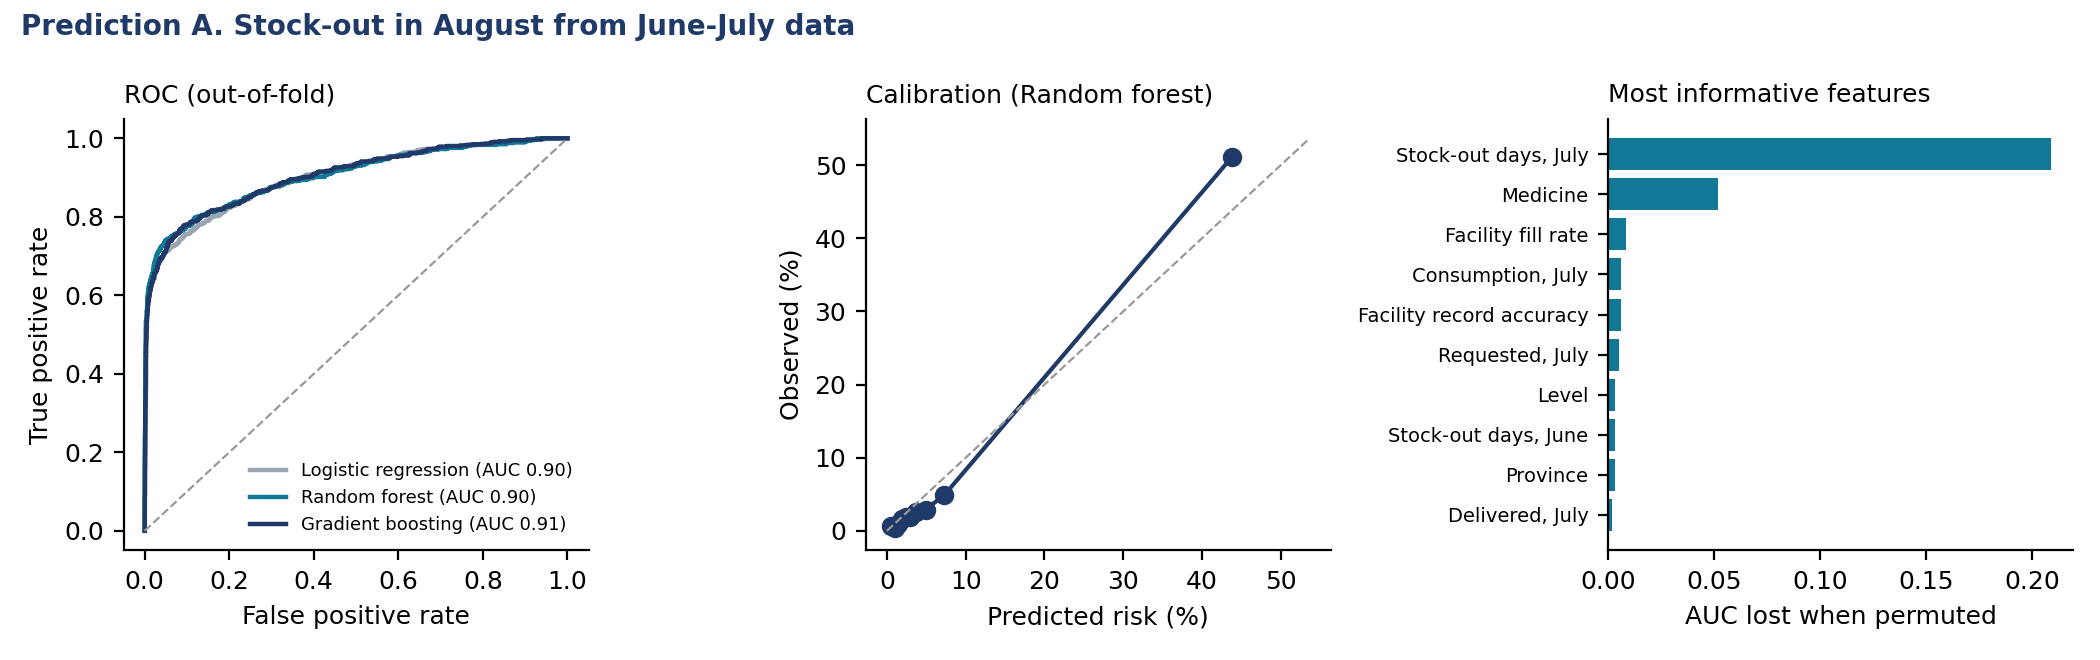
\includegraphics[width=0.94\linewidth]{fig_pred_august.png}\caption*{\small Figure 8. Prediction A: ROC, calibration and feature importance.}\end{figure}
\begin{figure}[htbp]\centering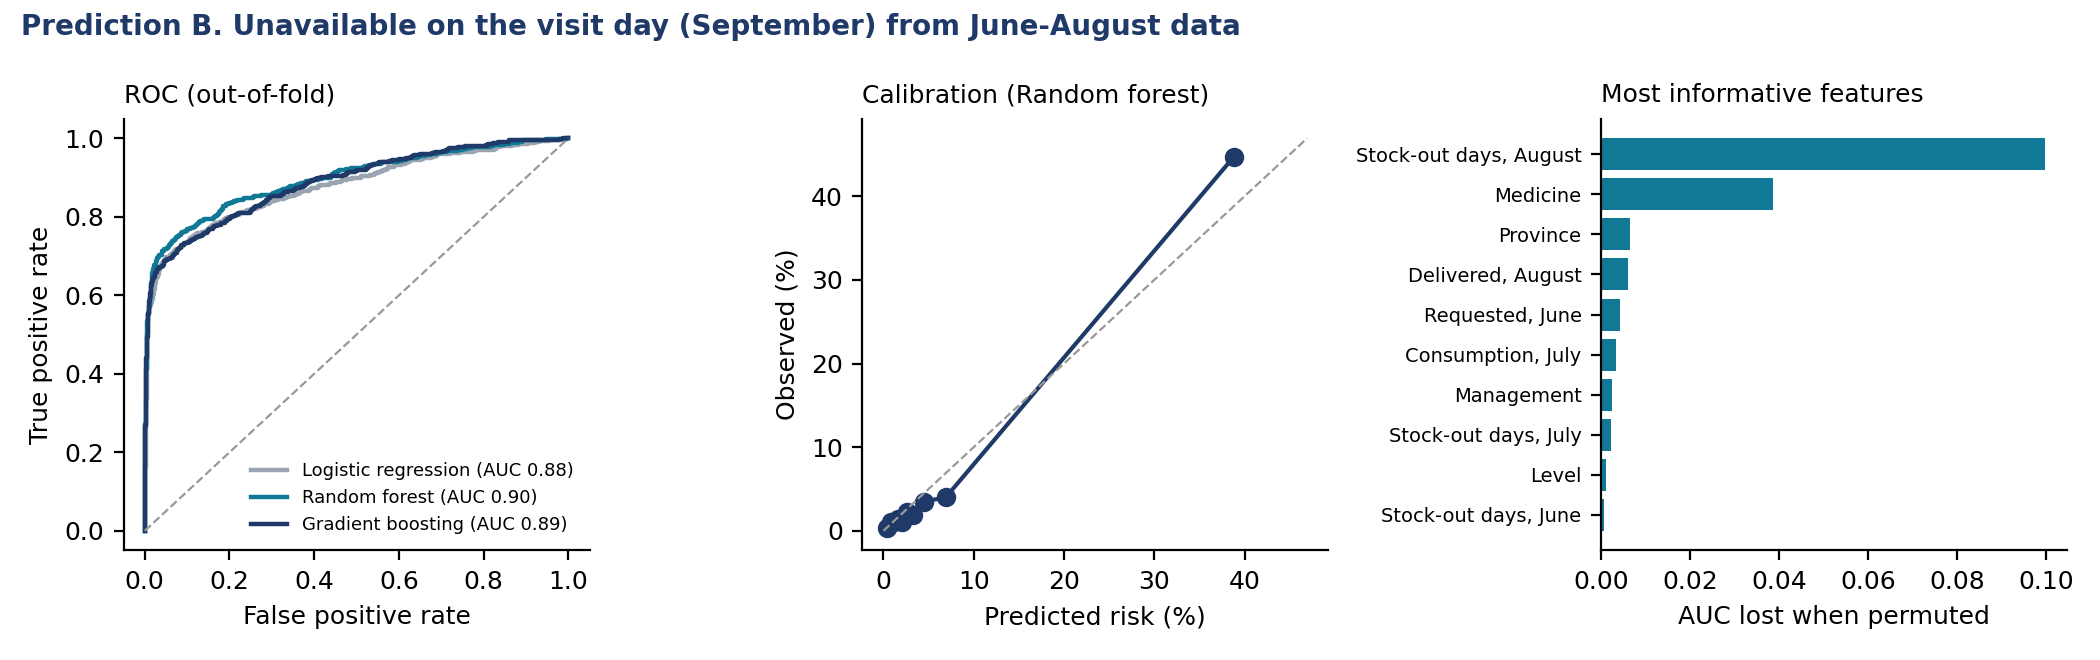
\includegraphics[width=0.94\linewidth]{fig_pred_visit.png}\caption*{\small Figure 9. Prediction B: ROC, calibration and feature importance.}\end{figure}
{\footnotesize\setlength{\tabcolsep}{3pt}
\begin{longtable}{>{\raggedright\arraybackslash}p{0.399\linewidth}>{\raggedright\arraybackslash}p{0.183\linewidth}>{\raggedright\arraybackslash}p{0.183\linewidth}>{\raggedright\arraybackslash}p{0.205\linewidth}}
\rowcolor{navy}\textbf{\color{white}Approach} & \textbf{\color{white}Pairs flagged} & \textbf{\color{white}Precision} & \textbf{\color{white}Recall} \\
\endhead
A: rule ''out in July'' & 6.3\% & 72.8\% & 66.7\% \\
\rowcolor{band}A: Random forest, same flag rate & 6.3\% & 71.6\% & 65.7\% \\
A: Random forest, top 10\% risk & 10.0\% & 51.1\% & 74.1\% \\
\rowcolor{band}B: rule ''out in July'' & 6.3\% & 49.2\% & 50.8\% \\
B: Random forest, same flag rate & 6.3\% & 65.5\% & 67.6\% \\
\rowcolor{band}B: Random forest, top 10\% risk & 10.0\% & 44.7\% & 73.1\% \\
\multicolumn{4}{p{0.97\linewidth}}{\scriptsize\itshape Precision: share of flagged pairs that stocked out. Recall: share of stock-outs flagged.}\\
\end{longtable}}
\textbf{Interpretation.} All three models discriminate well (AUC about 0.90 for August stock-outs and 0.90 for the visit day), and the random forest is well calibrated. Most of this comes from persistence: July stock-out days are by far the most informative feature, and for August the simple rule ''flag what was out in July'' performs as well as the model at the same flag rate. The models add value in two ways. First, they rank risk among pairs that were not out in July (AUC 0.73 for new August stock-outs; 0.81 for the visit day), using the medicine, consumption, requests and the facility's fill rate and record accuracy. Second, for the visit-day outcome the model beats the rule clearly at the same flag rate (precision 65.5\% against 49.2\%). Flagging the top 10\% of pairs by predicted risk captures about 74.1\% of next-month stock-outs with a 7.4-fold lift over random selection. A monthly early-warning list built from eLMIS data in this way is feasible; it should be validated on a later period before use, because three months is a short history.

\section{Discussion}
\subsection{Main messages}
\begin{itemize}\item \textbf{Availability is high by regional standards but uneven.} The managed-product figure (93.7\%) and the expected-medicine figure (87.8\%) are well above typical African public-sector values. The national weighted figure for expected medicines (77.7\%) is lower because health posts, which are most of Rwanda's facilities, do not stock many of the medicines the EML authorises for them.
\item \textbf{Order fulfilment is a lever with a measurable effect.} Nil-filled requisitions multiply the odds of next-month stock-out about 7.6-fold. This is the most actionable result for RMS, and it echoes evidence that order fulfilment and inventory policy, more than facility traits, drive stock-outs [Leung 2016; Mohan 2024].
\item \textbf{Stock problems are medicine- and pipeline-specific.} Facilities and districts explain little of the variation in availability and stock-outs, and there is no regional clustering. National quantification for the essential-medicines pipeline (insulin, thiamine, HIV test kits, paediatric RHZ) matters as much as facility mentorship.
\item \textbf{Record accuracy is the facility-level weakness, and it has slipped.} 56.1\% exact match is well below the 85\% QMIA reported for 2019 [Kigenza 2023], and eBuzima sites are markedly worse. This is where facility mentorship pays off.
\item \textbf{Antibiotic use is the main prescribing concern}, while generic and EML prescribing are excellent.
\item \textbf{The last mile to CHWs is the weak link in community supply.} Health centres hold stock their CHWs lack.
\end{itemize}
\subsection{Strengths and limitations}
\begin{itemize}\item \textbf{Strengths:} national coverage of all levels; linked stock, prescription and CHW data; confidence intervals and design effects that account for clustering; a temporally ordered test of order fulfilment; predictive models validated by facility-grouped cross-validation.
\item \textbf{Cross-sectional design.} Except for the lagged panel, associations are not causal.
\item \textbf{Short history.} Three months (June-August) limit trend and prediction; the models should be revalidated on later months.
\item \textbf{Weights.} Health posts were sampled purposively; weighted national figures that include them should be read as indicative.
\item \textbf{Self-report.} RMS availability and some quantities are facility-reported; consumption may be under-recorded where dispensing is not captured.
\item \textbf{Prescription design.} Prescribers write what the pharmacy holds, so unserved rates understate unmet need; there is no outpatient/inpatient flag.
\item \textbf{Zoning.} Cleaning rule S10 uses a partly inferred zoning list that differs from the published deployment plan for some districts [Muvunyi 2025].
\end{itemize}
\section{Recommendations}
\begin{itemize}\item \textbf{RMS: treat a nil-filled order as an alert.} Track requisitions delivered at 0\% and expedite or substitute within the month; report the share monthly by hub.
\item \textbf{Facilities: never skip a requisition cycle} for a managed medicine, even when stock looks sufficient; a missed order raises the odds of a stock-out next month about 2.6-fold.
\item \textbf{Build a monthly stock-out early-warning list} from eLMIS: pairs out last month plus the model's top-risk pairs, sent to RMS branches and district pharmacists.
\item \textbf{Focus QMIA mentorship on record reconciliation} at health centres using eBuzima, and at PPP facilities; aim to restore the 85\% accuracy of 2019.
\item \textbf{Use the facility profiles to tailor support:} redistribution for overstocked sites, RMS follow-up for weak-resupply sites, quantification support for frequent-stock-out sites.
\item \textbf{Strengthen health centre-to-CHW resupply}, especially ORS and zinc as a pair and amoxicillin in Kigali City; consider resupply at the monthly CHW meeting.
\item \textbf{Antimicrobial stewardship in primary care:} feed back antibiotic prescribing rates by facility and prescriber, starting with health centres and general practitioners.
\item \textbf{Report weighted estimates with confidence intervals} in the national report, and flag district values whose intervals include the national figure.
\item \textbf{Confirm the official MFT zoning list} and rerun the zoning rule and these analyses.
\end{itemize}
\section{References}
\begin{enumerate}[leftmargin=1.5em]\small\item Bizimana T, Kayumba PC, Heide L. Prices, availability and affordability of medicines in Rwanda. PLoS One. 2020;15(8):e0236411.
\item Cameron A, Ewen M, Ross-Degnan D, Ball D, Laing R. Medicine prices, availability, and affordability in 36 developing and middle-income countries: a secondary analysis. Lancet. 2009;373:240-249.
\item Chandani Y, Andersson S, Heaton A, et al. Making products available among community health workers: evidence for improving community health supply chains from Ethiopia, Malawi, and Rwanda. J Glob Health. 2014;4(2):020405.
\item Chandani Y, Duffy M, Lamphere B, et al. Quality improvement practices to institutionalize supply chain best practices for iCCM: evidence from Rwanda and Malawi. Res Social Adm Pharm. 2017;13(6):1095-1109.
\item Choi Y, Ametepi P. Comparison of medicine availability measurements at health facilities: evidence from Service Provision Assessment surveys in five sub-Saharan African countries. BMC Health Serv Res. 2013;13:266.
\item Gakinahe GU, Rutungwa E, Mbonyinshuti F, Kayitare E. Availability of antimalarial medicines and inventory management at the community level: a case study of Bugesera district in Rwanda. BMC Health Serv Res. 2024;24:136.
\item Kabera JC, Mukanyangezi MF. Influence of inventory management practices on the availability of emergency obstetric drugs in Rwandan public hospitals. BMC Health Serv Res. 2024;24.
\item Kigenza R, Nsengiyumva E, Sabagirirwa V. The Quality Management Improvement Approach: successes and lessons learned from a workforce development intervention in Rwanda's health supply chain. Glob Health Sci Pract. 2023;11(1):e2200295.
\item Kuwawenaruwa A, Wyss K, Wiedenmayer K, Metta E, Tediosi F. The effects of medicines availability and stock-outs on household's utilization of healthcare services in Dodoma region, Tanzania. Health Policy Plan. 2020;35(3):323-333.
\item Leung NHZ, Chen A, Yadav P, Gallien J. The impact of inventory management on stock-outs of essential drugs in sub-Saharan Africa: secondary analysis of a field experiment in Zambia. PLoS One. 2016;11(5):e0156026.
\item Manirakiza A, et al. Evaluating drug use patterns among paediatric outpatients in Burundi. J Pharm Policy Pract. 2024;17(1):2312369.
\item Masters SH, Burstein R, DeCenso B, et al. Pharmaceutical availability across levels of care: evidence from facility surveys in Ghana, Kenya, and Uganda. PLoS One. 2014;9(12):e114762.
\item Mbonyinshuti F, Nkurunziza J, Niyobuhungiro J, Kayitare E. The prediction of essential medicines demand: a machine learning approach using consumption data in Rwanda. Processes. 2022;10(1):26.
\item Mekonen ZT, Cho DJ, Fenta TG. Logistics Management Information System (LMIS) for health commodities at public health facilities in Amhara National Regional State of Ethiopia: a data quality evaluation survey. J Multidiscip Healthc. 2025;18:255-266.
\item Mohan S, Mangal TD, Colbourn T, et al. Factors associated with medical consumable availability in level 1 facilities in Malawi: a secondary analysis of a facility census. Lancet Glob Health. 2024;12(6):e1027-e1037.
\item Mukundiyukuri JP, Irakiza JJ, Nyirahabimana N, et al. Availability, costs and stock-outs of essential NCD drugs in three rural Rwandan districts. Ann Glob Health. 2020;86(1):123.
\item Muvunyi CM, Gashema P, Mbituyumuremyi A, et al. Strategies for mitigating emerging artemisinin-based antimalarial drug resistance in Rwanda. BMJ Glob Health. 2025;10(10):e020884.
\item Ofori-Asenso R, Brhlikova P, Pollock AM. Prescribing indicators at primary health care centers within the WHO African region: a systematic analysis (1995-2015). BMC Public Health. 2016;16:724.
\item Shabangu K, Suleman F. Medicines availability at a Swaziland hospital and impact on patients. Afr J Prim Health Care Fam Med. 2015;7(1):829.
\item Uwimana A, Legrand E, Stokes BH, et al. Emergence and clonal expansion of in vitro artemisinin-resistant Plasmodium falciparum kelch13 R561H mutant parasites in Rwanda. Nat Med. 2020;26(10):1602-1608.
\item World Health Organization. How to investigate drug use in health facilities: selected drug use indicators. WHO/DAP/93.1. Geneva: WHO; 1993.
\item Zupko RJ, Nguyen TD, Ngabonziza JCS, et al. Modeling policy interventions for slowing the spread of artemisinin-resistant pfkelch R561H mutations in Rwanda. Nat Med. 2023;29(11):2775-2784.
\end{enumerate}
\end{document}